\ifx\wholebook\relax \else

\documentclass[b5paper]{ctexart}
\usepackage[nomarginpar
  %, margin=.5in
]{geometry}

\addtolength{\oddsidemargin}{-0.05in}
\addtolength{\evensidemargin}{-0.05in}
\addtolength{\textwidth}{0.1in}

\usepackage[cn]{../../../prelude}

\setcounter{page}{1}

\begin{document}

\title{列表}

\author{刘新宇
\thanks{{\bfseries 刘新宇} \newline
  Email: liuxinyu95@gmail.com \newline}
  }

\maketitle
\fi

\markboth{列表}{基本算法}

\ifx\wholebook\relax
\chapter{列表}
\numberwithin{Exercise}{chapter}
\fi

\section{简介}
\label{introduction}

列表和数组是构建其它复杂数据结构的基石。它们都可以看作是容纳若干元素的容器。数组通常是一组连续的存储区域。每个存储单元由一个数字索引。这个数字叫作地址或者位置。数组的大小是有限的,通常需要在使用前预先确定。与数组不同,列表的大小无需预先确定,可以随时加入新元素。我们可以从头到尾依次遍历列表中的元素。特别在函数式环境中,列表相关算法对于计算和逻辑的控制起着关键作用\footnote{在更底层,lambda演算作为和图灵机等价的计算模型更为基础\cite{mittype}, \cite{unplugged}。}。对于已经熟悉映射(map),过滤(filter),叠加(fold)等算法的读者,可以跳过这一章,直接从第二章开始阅读。

\section{定义}
\index{列表!定义}

列表又称单向链表,是一种递归的数据结构。其定义如下:

\begin{itemize}
\item 一个\textbf{列表}或者为空,记为 $\nil$或NIL;
\item 或者包含一个元素和一个\textbf{列表}。
\end{itemize}

图\ref{fig:list-example}描述了一个由若干节点组成的列表。每个节点包含两部分,一个元素(也称作key)和一个子列表。指向子列表的引用通常叫作next。最后一个节点中的子列表为空,记为‘NIL’。

\begin{figure}[htbp]
  \centering
    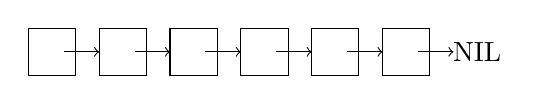
\begin{tikzpicture}[scale=3]
    \foreach \x in {-2, -1.7, ..., -0.4} {
      \draw (\x cm, 1cm) +(-0.1, -0.1) rectangle ++(0.1, 0.1);
      \draw[->] (\x cm, 1cm) +(0.05, 0) -- +(0.2, 0);
    }
    \draw (-0.2cm, 1cm) node {NIL};
    \end{tikzpicture}
  \caption{由节点组成的列表}
  \label{fig:list-example}
\end{figure}

每个节点要么链接到下一个节点上,要么指向NIL。通常使用复合数据结构\footnote{多数情况下,列表中元素有着共同的类型。有些环境(如Lisp)支持包含不同数据类型的列表。}定义链表,例如:

\lstset{frame=single}
\begin{lstlisting}[language=Bourbaki]
struct List<A> {
    A key
    List<A> next
}
\end{lstlisting}

\index{列表!空} \index{列表!判空}

这里需要对“空”列表的概念加以说明。很多传统的编程环境支持空引用null概念,因此存在两种不同的方法表示空列表。一种直接使用空引用null(或NIL);另一种创建一个列表,但不填入任何元素,通常表示为\texttt{[]}。在实现上,空引用无需占用内存,但\texttt{[]}则需要分配内存。本书使用符号$\varnothing$表示抽象的空列表、空集、空容器。

\subsection{析趣}
\index{列表!头} \index{列表!尾} \index{列表!构造} \index{列表!cons}

给定一个非空列表$L$,我们定义两个函数来分别获取头一个元素和子列表。它们通常被命名为$first(L)$和$rest(L)$,或者$head(L)$和$tail(L)$\footnote{在Lisp中,由于历史原因,它们被命名为\texttt{car}和\texttt{cdr}用以代表当时机器中的寄存器\cite{SICP}}。反之,我们可以从一个元素$x$和列表$xs$(可为空)构造出另一个列表,记为$x : xs$。这一构造过程也叫作\texttt{cons}。我们有如下关系:

\be
\begin{cases}
head(x:xs) & = x \\
tail(x:xs) & = xs
\end{cases}
\ee

对于非空列表$X$,我们也用$x_1$表示头一个元素,用$X'$表示剩余列表,即$X = [x_1, x_2, x_3, ...]$,$X' = [x_2, x_3, ...]$。

\begin{Exercise}
\Question{对于元素类型为$A$的列表,如果能够判断任何两个元素$x, y \in A$是否相等,定义一个算法来判断两个列表是否相等。}
\end{Exercise}

\subsection{列表的基本操作}
\index{列表!长度}
根据定义,我们可以递归地计算列表的长度:空列表的长度为0,而非空列表的长度是除去第一个元素的子列表长度加一。

\be
\begin{array}{rcl}
length(\nil) & = & 0 \\
length(L) & = & 1 + length(L')
\end{array}
\ee

为了计算长度,我们从头到尾遍历列表。其时间复杂度$O(n)$,其中$n$是元素个数。为了避免反复计数,我们可以将长度存储在一个变量中,并在增加或删除元素时更新这一变量。下面是迭代计算长度的实现:

\begin{algorithmic}[1]
\Function{Length}{L}
  \State $n \gets 0$
  \While{$L \neq $ NIL}
    \State $n \gets n + 1$
    \State $L \gets $ \Call{Next}{$L$}
  \EndWhile
  \State \Return $n$
\EndFunction
\end{algorithmic}

在上下文不和绝对值混淆的情况下,我们也使用$|L|$来表示列表$L$的长度。

\subsection{索引}
\index{列表!索引(get at)}

数组支持在常数时间随机访问任意位置$i$的元素。但列表需要前进$i$步才能到达元素所在位置。

\be
getAt(i,\ x:xs) = \begin{cases}
  i = 0: & x \\
  i \neq 0: & getAt(i - 1, xs) \\
\end{cases}
\ee

为了从一个非空列表中获取第$i$个元素:
\begin{itemize}
\item 若$i$为0,结果为列表中的头一个元素;
\item 否则,结果为子列表中的第$i-1$个元素。
\end{itemize}

我们故意没有处理空列表的情况。如果传入$\nil$,此时的行为是未定义的。因此$i$越界时的行为也是未定义的。若$i > |L|$,通过递归,最终转化为访问空列表的第$i - |L|$的情况。另一方面,若$i < 0$,继续减一将使得它更偏离0,最终转化为访问空列表的某个负索引位置的情况。

由于需要前进$i$步,索引算法的时间复杂度为$O(i)$。下面是对应的迭代实现:

\begin{algorithmic}[1]
\Function{Get-At}{$i, L$}
  \While{$i \neq 0$}
    \State $L \gets $ \Call{Next}{$L$}  \Comment{$L$ = NIL时出错}
    \State $i \gets i - 1$
  \EndWhile
  \State \Return \Call{First}{$L$}
\EndFunction
\end{algorithmic}

\begin{Exercise}
\Question{在\textproc{Get-At}($i, L$)的迭代实现中,$L$为空会怎样?$i$越界时会怎样?}
\end{Exercise}

\subsection{末尾元素}
\index{列表!末尾元素} \index{列表!init}

存在一对和first/rest对称的操作,称为last/init。对于非空列表$X = [x_1, x_2, ..., x_n]$,函数$last$返回末尾元素$x_n$,而$init$返回子列表$[x_1, x_2, ..., x_{n-1}]$。虽然这两对操作左右对称,但last/init需要遍历列表,因而是线性时间的。

当获取列表$X$的末尾元素时:

\begin{itemize}
\item 如果列表只含有一个元素$[x_1]$,则$x_1$就是末尾元素;
\item 否则,结果为子列表$X'$的末尾元素。
\end{itemize}

\be
\begin{array}{rcl}
last([x]) & = & x \\
last(x:xs) & = & last(xs) \\
\end{array}
\ee

类似地,当获取除去末尾元素的子列表时:

\begin{itemize}
\item 如果列表只含有一个元素$[x_1]$,结果为空$[\ ]$;
\item 否则,我们递归地从子列表$X'$中获取除去末尾元素的剩余部分,然后将$x_1$附加在前面。
\end{itemize}

\be
\begin{array}{rcl}
init([x]) & = & [\ ] \\
init(x:xs) & = & x : init(xs) \\
\end{array}
\ee

这两个算法中都没有处理空列表的情况,当传入$\nil$时,其行为是为定义的。下面是相应的迭代实现。

\begin{algorithmic}[1]
\Function{Last}{$L$}
  \State $x \gets $ NIL
  \While{$L \neq$ NIL}
    \State $x \gets $ \Call{First}{$L$}
    \State $L \gets $ \Call{Rest}{$L$}
  \EndWhile
  \State \Return $x$
\EndFunction
\Statex
\Function{Init}{$L$}
  \State $L' \gets $ NIL
  \While{\Call{Rest}{$L$} $\neq$ NIL} \Comment{$L$为NIL时出错}
    \State $L' \gets$ \textproc{Cons}(\Call{First}{$L$}, $L'$)
    \State $L \gets $ \Call{Rest}{$L$}
  \EndWhile
  \State \Return \Call{Reverse}{$L'$}
\EndFunction
\end{algorithmic}

这一算法一边向尾部前进么,一边通过cons累积init的结果。但是这样产生的列表是逆序的,因此最后需要将结果倒转过来(定义见第\ref{sec:reverse}节)。本章练习中有一道题目,提问是否可以用append代替cons。

\subsection{反向索引}
\index{列表!反向索引} \index{列表!rindex}

$last()$是反向索引的一种特例。更一般的形式是获取列表中的倒数第$i$个元素。最直接的思路是遍历两次:第一次获取列表长度$n$,第二次获取第$n - i - 1$个元素:

\be
  lastAt(i, L) = getAt(|L| - i - 1, L)
\ee

更好的解法是使用两个指针$p_1$和$p_2$,它们相距$i$步,即$rest^i(p_2) = p_1$,其中$rest^i(p_2)$表示重复执行函数$rest()$总共$i$次。也就是说,从$p_2$前进$i$步就可到达$p_1$。$p_2$一开始指向链表的头部,然后同时向前移动它们,直到$p_1$到达链表的尾部。此时指针$p_2$恰好指向倒数第$i$个元素。图\ref{fig:list-rindex}描述了这一方法。由于$p_1, p_2$框出一个窗口,这一方法也称作滑动窗口法。

\begin{figure}[htbp]
    \centering
    \subcaptionbox{$p_2$开始时指向表头,它在指针$p_1$之后,距离$i$步。}{\includegraphics[scale=0.8]{img/list-rindex.ps}} \\
    \subcaptionbox{当$p_1$到达表尾时,$p_2$恰好指向从右数第$i$个元素。}{\includegraphics[scale=0.8]{img/list-rindex-2.ps}}
    \caption{双指针框出一个滑动窗口}
    \label{fig:list-rindex}
\end{figure}

\begin{algorithmic}[1]
\Function{Last-At}{$i, L$}
  \State $p \gets L$
  \While{$i > 0$}
    \State $L \gets $ \Call{Rest}{$L$} \Comment{越界时出错}
    \State $i \gets i - 1$
  \EndWhile
  \While{\Call{Rest}{$L$} $\neq$ NIL}
    \State $L \gets$ \Call{Rest}{$L$}
    \State $p \gets$ \Call{Rest}{$p$}
  \EndWhile
  \State \Return \Call{First}{$p$}
\EndFunction
\end{algorithmic}

纯函数实现时不能直接更新指针,为此我们可以同时向前遍历$X = [x_1, x_2, ..., x_n]$和$Y = [x_i, x_{i+1}, ..., x_n]$,其中$Y$是除去前$i-1$个元素后的子列表。

\begin{itemize}
\item 如果$Y$中仅含有一个元素,$[x_n]$,则倒数第$i$个元素就是表头$x_n$;
\item 否则,我们同时从$X$和$Y$中各丢弃一个元素,然后递归地检查列表$X'$和$Y'$。
\end{itemize}

\be
lastAt(i, X) = slide(X, drop(i, X))
\ee

其中数函$slide(X, Y)$同时丢弃两个列表的头部:

\be
\begin{array}{rcl}
slide(x:xs,\ [y]) & = & x \\
slide(x:xs,\ y:ys) & = & slide(xs, ys) \\
\end{array}
\ee

函数$drop(m, X)$丢弃列表$X$中的前$m$个元素,我们可以通过从表头前进$m$步实现:

\be
\begin{array}{rcl}
drop(0,\ X) & = & X \\
drop(m,\ \nil) & = & \nil \\
drop(m,\ x:xs) & = & drop(m - 1, xs) \\
\end{array}
\ee

\begin{Exercise}
\Question{在\textproc{Init}算法中,我们可以用\textproc{Append}($L'$, \textproc{First}($L$))来替换cons么?}
\Question{在\textproc{Last-At}算法中,如何处理空列表和越界的情况?}
\end{Exercise}

\subsection{更改}
\index{列表!更改}

更改操作包括添加、插入、更新、删除。某些函数式环境在实现时创建一新列表,而原列表保持(persist)不变,并在适当的时候释放原始列表(\cite{okasaki-book},第2章)。

\subsubsection{添加}
\index{列表!添加}

添加称为Append,它是和cons对称的操作。一个在表头增加元素,一个在末尾增加元素。因此添加也被称作snoc(将cons反过来拼写)。由于要遍历到列表尾部进行操作,所以其复杂度为$O(n)$,其中$n$是列表的长度。为了避免反复遍历,我们可以将尾部位置存储下来,并随着列表变化进行更新。

\be
\begin{array}{rcl}
append(\nil, x) & = & [x] \\
append(y:ys, x) & = & y : append(ys, x) \\
\end{array}
\ee

\begin{itemize}
\item 向空列表添加$x$,结果为$[x]$;
\item 否则,将$x$添加到子列表的末尾。
\end{itemize}

对应的迭代实现如下:

\begin{algorithmic}[1]
\Function{Append}{$L, x$}
  \If{$L = $ NIL}
    \State \Return \Call{Cons}{$x$, NIL}
  \EndIf
  \State $H \gets L$ \Comment{save the head}
  \While{\Call{Rest}{$L$} $\neq$ NIL}
    \State $L \gets$ \Call{Rest}{$L$}
  \EndWhile
  \State \Call{Rest}{$L$} $\gets$ \Call{Cons}{$x$, NIL}
  \State \Return $H$
\EndFunction
\end{algorithmic}

更新\textproc{Rest}的过程通常实现为对\texttt{next}引用的改写,如下面的例子代码:

\begin{lstlisting}[language=Bourbaki]
List<A> append(List<A> xs, T x) {
    if (xs == null) {
        return cons(x, null)
    }
    List<A> head = xs
    while (xs.next != null) {
        xs = xs.next
    }
    xs.next = cons(x, null)
    return head
}
\end{lstlisting}

\begin{Exercise}
\Question{在列表的定义中增加一个尾部tail变量,将添加算法优化为常数时间。}
\Question{何时应该更新tail变量?对性能有何影响?}
\end{Exercise}

\subsubsection{修改}
\index{列表!修改}

和$getAt$类似,我们需要移动到列表中的指定位置以修改元素。定义函数$setAt(i, x, L)$为:

\begin{itemize}
\item 若$i = 0$,要修改的是头部元素,结果为$x : L'$;
\item 否则,递归地修改子列表$L'$中的第$i - 1$个元素。
\end{itemize}

\be
\begin{array}{rcl}
setAt(0, x,\ y:ys) & = & x : ys \\
setAt(i, x,\ y:ys) & = & y : setAt(i - 1, x, ys) \\
\end{array}
\ee

这一算法的时间复杂度为$O(i)$,其中$i$是要修改的位置。

\begin{Exercise}
\Question{在$setAt$中,如何处理空列表和越界的情况?}
\end{Exercise}

\subsubsection{插入}
\index{列表!插入}

列表插入有两个不同的含义:一个是在指定位置插入一个元素,记为$insert(i, x, L)$,其实现和$setAt$类似;另一含义是在一已序列表中插入一个元素,使得结果仍然是已序的。

为了插入元素$x$,需要先前进$i$步到达插入位置。然后用$x$和后续子列表构造一个新列表,再和前$i$个元素附链接起来。

\begin{itemize}
\item 若$i = 0$,插入就转变成了cons,结果为$x : L$;
\item 否则,递归地将$x$插入到子列表$L'$的第$i-1$个位置,并将原头部元素附加在前面。
\end{itemize}

\be
\begin{array}{rcl}
insert(0, x,\ L) & = & x : L \\
insert(i, x,\ y:ys) & = & x : insert(i - 1, x, ys) \\
\end{array}
\ee

当$i$超过列表的长度时,我们可以将其视作添加,见本节习题。下面是相应的迭实现:

\begin{algorithmic}[1]
\Function{Insert}{$i, x, L$}
  \If{$i = 0$}
    \State \Return \Call{Cons}{$x, L$}
  \EndIf
  \State $H \gets L$
  \State $p \gets L$
  \While{$i > 0$ and $L \neq$ NIL}
    \State $p \gets L$
    \State $L \gets $ \Call{Rest}{$L$}
    \State $i \gets i - 1$
  \EndWhile
  \State \Call{Rest}{$p$} $\gets$ \Call{Cons}{$x, L$}
  \State \Return $H$
\EndFunction
\end{algorithmic}

如果列表$L = [x_1, x_2, ..., x_n]$已序,即对任何位置$1 \leq i \leq j \leq n$,有$x_i \leq x_j$。这里的小于号$\leq$的含义是抽象的,它可以代表任何有序的比较,包括$\geq$(降序)、集合的包含关系等。我们可以设计一个算法,使得新元素$x$插入$L$后,结果列表仍然有序。

\begin{itemize}
\item 若$L$为空或者$x$小于$L$的头部元素,结果为$x : L$;
\item 否则,我们递归地将元素$x$插入到子列表$L'$中。
\end{itemize}

\be
\begin{array}{rcl}
insert(x,\ \nil) & = & [x] \\
insert(x,\ y : ys) & = & \begin{cases}
  x \leq y : & x : y : ys \\
  otherwise : & y : insert(x, ys) \\
  \end{cases}
\end{array}
\ee

由于要逐一比较元素,插入的时间复杂度为$O(n)$,其中$n$是长度。对应的迭代实现如下:

\begin{algorithmic}[1]
\Function{Insert}{$x, L$}
  \If{$L = $ NIL or $x <$ \Call{First}{$L$}}
    \State \Return \Call{Cons}{$x, L$}
  \EndIf
  \State $H \gets L$
  \While{\Call{Rest}{$L$} $\neq $ NIL and \textproc{First}(\Call{Rest}{$L$}) $< x$}
    \State $L \gets $ \Call{Rest}{$L$}
  \EndWhile
  \State \Call{Rest}{$L$} $\gets$ \textproc{Cons}($x$, \Call{Rest}{$L$})
  \State \Return $H$
\EndFunction
\end{algorithmic}

\label{sec:isort}
利用这一线性时间的按序插入操作,我们可以实现插入排序:逐一将元素按序插入到一个空列表中。由于每次按序插入都是线性的,所以这一排序的复杂度为$O(n^2)$。

\be
\begin{array}{rcl}
sort(\nil) & = & \nil \\
sort(x:xs) & = & insert(x, sort(xs)) \\
\end{array}
\ee

这是一个递归算法:先递归地将子列表排序,然后把第一个元素按序插入。我们可以消除递归,实现一个迭代算法:逐一从链表中取出元素并按序插入到结果中:

\begin{algorithmic}[1]
\Function{Sort}{$L$}
  \State $L' \gets$ NIL
  \While{$L \neq$ NIL}
    \State $L' \gets$ \textproc{Insert}(\Call{First}{$L$}, $L'$)
    \State $L \gets$ \Call{Rest}{$L$}
  \EndWhile
  \State \Return $L'$
\EndFunction
\end{algorithmic}

在循环中的任何时刻,结果列表都是已序的。和递归实现相比,它们有一个本质不同:前者从右向左处理列表,而后者从左向右处理。我们稍后将在“尾递归”\ref{sec:tail-call}一节中讲述如何消除这一差异。第3章详细介绍插入排序,包括性能分析和优化。

\begin{Exercise}
\Question{当插入位置越界时,将其按照添加来处理。}
\Question{针对数组实现插入算法,插入位置$i$后的所有元素需要向后移动一个位置。}
\Question{只使用小于$<$比较实现插入排序。}
\end{Exercise}

\subsubsection{删除}
\index{列表!删除}

和插入类似,删除也有两种含义:一种是在指定位置删除元素;另一个是查找某个值的元素并删除。前者定义为$delAt(i, L)$,后者定义为$delete(x, L)$。

为了删除位置$i$上的元素,我们首先前进$i$步到达目标位置,然后跳过一个元素,将剩余部分连接起来。

\begin{itemize}
\item 若列表$L$为空,则结果为空列表;
\item 若$i = 0$,要删除的是头部元素,结果为$L'$;
\item 否则,递归地从子列表$L'$中删除第$i-1$个元素,然后将原列表头部附加在前。
\end{itemize}

\be
\begin{array}{rcl}
delAt(i,\ \nil) & = & \nil \\
delAt(0,\ x:xs) & = & xs \\
delAt(i,\ x:xs) & = & x : delAt(i - 1, xs) \\
\end{array}
\ee

由于需要前进$i$步后执行删除,这一算法的时间复杂度为$O(i)$。下面是相应的迭代实现:

\begin{algorithmic}[1]
\Function{Del-At}{$i, L$}
  \State $S \gets$ \Call{Cons}{$\perp, L$} \Comment{辅助节点}
  \State $p \gets S$
  \While{$i > 0$ and $L \neq$ NIL}
    \State $i \gets i - 1$
    \State $p \gets L$
    \State $L \gets $ \Call{Rest}{$L$}
  \EndWhile
  \If{$L \neq$ NIL}
    \State \Call{Rest}{$p$} $\gets$ \Call{Rest}{$L$}
  \EndIf
  \State \Return \Call{Rest}{$S$}
\EndFunction
\end{algorithmic}

为了简化边界情况的处理,我们引入来一个辅助节点$S$,它包含一个特殊的值$\perp$,并接下来指向$L$。使用$S$,我们可以安全地切除$L$中的任何节点,包括头节点。最后,我们将$S$后继的部分作为结果返回,并丢弃$S$自身。

“查找并删除”的语义可以进一步细分为两种情况,一种是仅仅找到第一个出现的元素,并将其从列表中删除;另外一种是找到\underline{所有}等于指定值的元素,并将它们全部删除。后者是更加通用的情况,可以对第一种情况略作修改加以实现。我们将其作为练习留给读者。

我们按照“查找并删除”,而非“查找然后删除”来实现这一算法,通过一轮遍历完成查找和删除两个操作。

\begin{itemize}
\item 如果列表为空,则结果显然也是空列表;
\item 如果列表不为空,首先检查第一个元素,如果它恰好等于要删除的值,则结果等于列表的剩余部分;
\item 否则,我们取出第一个元素,然后递归地在剩余部分删除指定的值,然后在将取出的第一个元素放在这一结果的前面。
\end{itemize}

这一算法可以形式化为下面的定义。

\be
delete(L, x) = \left \{
  \begin{array}
  {r@{\quad:\quad}l}
  \phi & L = \phi \\
  L' & l_1 = x \\
  cons(l_1, delete(L', x)) & otherwise
  \end{array}
\right.
\ee

由于需要遍历列表以查找待删除的元素,这一算法的复杂度为线性时间。下面的Haskell例子程序实现了这一算法。其中第一个边界条件使用模式匹配来处理,其余两种情况由if-else表达式处理。

\lstset{language=Haskell}
\begin{lstlisting}[style=Haskell]
del [] _ = []
del (x:xs) y = if x == y then xs else x : del xs y
\end{lstlisting}

此前的命令式算法中,大都跳过了错误处理。但是“查找并删除”时,必须要处理待查找的值不存在的情况。

\begin{algorithmic}[1]
\Function{Delete}{$L, x$}
  \If{$L = \phi$} \Comment{空列表}
    \State \Return $\phi$
  \EndIf
  \If{\Call{First}{$L$} $= x$}
    \State $H \gets$ \Call{Rest}{$L$}
  \Else
    \State $H \gets L$
    \While{$L \neq \phi \land$ \Call{First}{$L$} $\neq x$} \Comment{列表不为空}
      \State $p \gets L$
      \State $L \gets$ \Call{Rest}{$L$}
    \EndWhile
    \If{$L \neq \phi$} \Comment{找到}
      \State \Call{Rest}{$p$} $\gets$ \Call{Rest}{$L$}
    \EndIf
  \EndIf
  \State \Return $H$
\EndFunction
\end{algorithmic}

如果列表为空,结果仍为空列表;否则,算法遍历列表直到发现一个元素等于待删除的值,或者到达列表末尾。如果找到了这样的元素,就将其从列表中去掉。下面的C++例子程序实现了这一算法。这里我们释放掉了被删除元素所占的存储空间。

\lstset{language=C++}
\begin{lstlisting}
template<typename T>
List<T>* del(List<T>* xs, T x) {
    List<T> *head, *prev;
    if (!xs)
        return xs;
    if (xs->key == x)
        head = xs->next;
    else {
        for (head = xs; xs && xs->key != x; xs = xs->next)
            prev = xs;
        if (xs)
            prev->next = xs->next;
    }
    if (xs) {
        xs->next = NULL;
        delete xs;
    }
    return head;
}
\end{lstlisting}

\subsubsection{连接}
\label{concat}
\index{列表!连接}

连接可以认为是添加操作的更一般形式,添加每次向列表尾部加入一个元素,而连接向列表尾部一次加入多个元素。

但是,如果通过多次添加来实现连接,则整体操作的性能不佳,为平方级别。考虑下面的实现。

\[
concat(L_1, L_2) = \left \{
  \begin{array}
  {r@{\quad:\quad}l}
  L_1 & L_2 = \phi \\
  concat(append(L_1, first(L_2)), rest(L_2)) & otherwise
  \end{array}
\right.
\]

每次添加都需要遍历到列表的尾部,一共需要$|L_2|$次遍历。总体性能为$O(|L_1| + (|L_1| + 1) + ... + (|L_1| + |L_2|)) = O(|L_1||L_2| + |L_2|^2)$。

与添加相比,链接操作的速度很快,为常数时间$O(1)$,我们可以只遍历$L_1$一次,然后将第二个列表链接到$L_1$的尾部。

\be
concat(L_1, L_2) = \left \{
  \begin{array}
  {r@{\quad:\quad}l}
  L_2 & L_1 = \phi \\
  cons(first(L_1), concat(rest(L_1), L_2)) & otherwise
  \end{array}
\right.
\ee

这一算法只通过一次遍历到达$L_1$的尾部,然后将第二个列表链接起来。因此总体性能为线性时间$O(|L_1|)$。

算法的描述如下。

\begin{itemize}
\item 若第一个列表为空,则连接的结果就是第二个列表;
\item 否则,我们将第二个列表连接到第一个列表中除去第一个元素外的剩余部分,然后再将第一个元素置于这一结果前。
\end{itemize}

大多数函数式环境提供了内置的函数或操作符来实现列表的连接操作,例如在ML语言家族中,\texttt{++}被用来连接两个列表。

\lstset{language=Haskell}
\begin{lstlisting}[style=Haskell]
[] ++ ys = ys
xs ++ [] = xs
(x:xs) ++ ys = x : xs ++ ys
\end{lstlisting}

这里我们加入了另外一种边界情况,如果第二个列表为空,我们无需遍历到第一个列表的尾部。连接结果为第一个列表。

在命令式环境中,通过在数据结构中增加一个尾指针,可以实现常数时间$O(1)$的连接操作。我们略过这种方法的实现。

若不使用尾指针,我们仍需遍历到第一个列表的尾部。

\begin{algorithmic}[1]
\Function{Concat}{$L_1, L_2$}
  \If{$L_1 = \phi$}
    \State \Return $L_2$
  \EndIf
  \If{$L_2 = \phi$}
    \State \Return $L_1$
  \EndIf
  \State $H \gets L_1$
  \While{\Call{Rest}{$L_1$} $\neq \phi$}
    \State $L_1 \gets$ \Call{Rest}{$L_1$}
  \EndWhile
  \State \Call{Rest}{$L_1$} $\gets L_2$
  \State \Return $H$
\EndFunction
\end{algorithmic}

下面的C++例子程序实现了列表的连接。

\lstset{language=C++}
\begin{lstlisting}
template<typename T>
List<T>* concat(List<T>* xs, List<T>* ys) {
    List<T>* head;
    if (!xs)
        return ys;
    if (!ys)
        return xs;
    for (head = xs; xs->next; xs = xs->next);
    xs->next = ys;
    return head;
}
\end{lstlisting}

\subsection{和与积}
\index{列表!和}
\index{列表!积}

\subsubsection{递归求和与求积}

对于数字列表,我们常常要计算和与积。它们的计算结构很类似。我们稍后会介绍如何抽象这样的计算结构。

为了计算\underline{列表中元素的和}:

\begin{itemize}
\item 若列表为空,则结果为0;
\item 否则,结果为第一个元素加上\underline{剩余元素的和}。
\end{itemize}

求和的描述可以形式化为下面的定义。

\be
sum(L) =  \left \{
  \begin{array}
  {r@{\quad:\quad}l}
  0 & L = \phi \\
  l_1 + sum(L') & otherwise
  \end{array}
\right.
\ee

但是,我们不能简单地将加法替换为乘法以获取列表中元素的积,否则结果总为0。我们需要定义空列表的积为1。

\be
product(L) = \left \{
  \begin{array}
  {r@{\quad:\quad}l}
  1 & L = \phi \\
  l_1 \times product(L') & otherwise
  \end{array}
\right.
\ee

下面的Haskell例子程序实现了和与积的计算。

\lstset{language=Haskell}
\begin{lstlisting}[style=Haskell]
sum [] = 0
sum (x:xs) = x + sum xs

product [] = 1
product (x:xs) = x * product xs
\end{lstlisting}

两个算法都需要遍历整个列表,因此它们的性能都为线性时间$O(n)$。

\subsubsection{尾递归}
\index{尾递归}
\index{尾调用}
\index{尾递归调用}

注意到无论是求和还是求积的算法都从右向左计算。我们可以修改它们的实现,从左向右\underline{累积计算}结果。求和时,结果从0开始累积,逐一将每个元素加到结果上,直到处理完全部列表。具体描述如下:

当通过求和累积结果时:
\begin{itemize}
\item 若列表为空,则累积结束,返回累积结果;
\item 否则,取出列表中的第一个元素,将其加到累积结果上,然后继续处理剩余的列表。
\end{itemize}

将这一描述形式化为定义,就可以得到另一种累加的算法。

\be
sum'(A, L) =  \left \{
  \begin{array}
  {r@{\quad:\quad}l}
  A & L = \phi \\
  sum'(A + l_1, L') & otherwise
  \end{array}
\right.
\ee

最终求和可以通过调用这一函数实现。我们传入0作为累加的起始值,同时传入待累加的列表。
\be
sum(L) = sum'(0, L)
\ee

这一改进除了将计算的顺序恢复为从左向右之外,还有一个重要的特点。观察函数$sum'(A, L)$的定义,我们发现它无需记录任何中间结果或者状态用于递归。所有的状态或者作为参数(例如$A$)传入接下来的递归调用,或者可以丢弃(例如列表中前面处理过的元素)。因此在实际的实现中,这样的递归函数可以进一步优化为循环,从而完全消除递归。

我们称这样的函数为“尾递归”(或“尾调用”),对其消除递归的优化称为“尾递归优化”\cite{wiki-tail-call}。顾名思义,这类函数中,递归发生在最后一步。尾递归优化可以极大地提高性能,并避免由于过深递归造成的调用栈溢出。

下面的Haskell例子程序给出了尾递归形式的求和与求积实现。

\lstset{language=Haskell}
\begin{lstlisting}[style=Haskell]
sum = sum' 0 where
    sum' acc [] = acc
    sum' acc (x:xs) = sum' (acc + x) xs

product = product' 1 where
    product' acc [] = acc
    product' acc (x:xs) = product' (acc * x) xs
\end{lstlisting}

在前面关于插入排序的部分,我们提到了函数式的实现从右向左对元素排序,我们也可以将其改为尾递归的形式。

\be
sort'(A, L) = \left \{
  \begin{array}
  {r@{\quad:\quad}l}
  A & L = \phi \\
  sort'(insert(l_1, A), L') & otherwise
  \end{array}
\right.
\ee

排序时,我们可以调用这一函数,传入一个空列表作为累积结果的起始值。
\be
sort(L) = sort'(\phi, L)
\ee

我们将它的具体实现作为练习留给读者。

作为本节的结尾,我们考虑一个有趣的题目,如何设计一个算法来高效地计算$b^n$?(参考\cite{SICP}中的1.16节。)

最直接的方法是从1开始重复乘以$b$共$n$次,这是一个线性时间$O(n)$的算法。

\begin{algorithmic}[1]
\Function{Pow}{$b, n$}
  \State $x \gets 1$
  \Loop{$n$ times}
    \State $x \gets x \times b$
  \EndLoop
  \State \Return $x$
\EndFunction
\end{algorithmic}

我们考虑如何改进它。考虑计算$b^8$的过程,上述算法经过前两次迭代,可以得到$x = b^2$的结果。此时,我们无需再次用$x$乘以$b$得到$b^3$,可以直接再次乘以$b^2$,从而得到$b^4$。然后再次乘方,就可以得到$(b^4)^2 = b^8$。这样总共只要循环3次,而不是8次。

若$n$恰好为2的整数次幂,即$n = 2^m$,其中$m$是非负整数,则根据这一思路,我们可以用下面的等式快速计算$b^n$。

\[
pow(b, n) =  \left \{
  \begin{array}
  {r@{\quad:\quad}l}
  b & n = 1 \\
  pow(b, \frac{n}{2})^2 & otherwise
  \end{array}
\right.
\]

我们可以扩展这一分而治之的想法,从而将$n$推广到任意的非负整数。

\begin{itemize}
\item 边界情况,$n$为0,结果显然为1;
\item 若$n$为偶数,我们将$n$减半,先计算$b^{\frac{n}{2}}$。然后在将这一结果平方。
\item 否则,$n$为奇数。因为$n-1$是偶数,我们可以先递归计算$b^{n-1}$,然后在将这一结果乘以$b$。
\end{itemize}

这一算法可以定义为下面的等式。

\be
pow(b, n) =  \left \{
  \begin{array}
  {r@{\quad:\quad}l}
  1 & n = 0 \\
  pow(b, \frac{n}{2})^2 & 2 | n \\
  b \times pow(b, n-1) & otherwise
  \end{array}
\right.
\ee

但是,这一算法并不能直接转换为尾递归的形式,原因是第二条递归调用。实际上,我们可以先将底数平方,然后在将指数减半。

\be
pow(b, n) =  \left \{
  \begin{array}
  {r@{\quad:\quad}l}
  1 & n = 0 \\
  pow(b^2, \frac{n}{2}) & 2 | n \\
  b \times pow(b, n-1) & otherwise
  \end{array}
\right.
\ee

通过这一修改,就可以将这一算法转换为尾递归形式了。我们通过等式$b^n = pow'(b, n, 1)$计算。

\be
pow'(b, n, A) =  \left \{
  \begin{array}
  {r@{\quad:\quad}l}
  A & n = 0 \\
  pow'(b^2, \frac{n}{2}, A) & 2 | n \\
  pow'(b, n-1, A \times b) & otherwise
  \end{array}
\right.
\ee

和最初的方法相比,我们把性能提高到了$O(\lg n)$。实际上这意思算法还可以继续改进。

如果我们将$n$表示成二进制数$n = (a_ma_{m-1}...a_1a_0)_2$,如果$a_i = 1$,我们清楚地知道,需要计算$b^{2^i}$。这和二项式堆的情况很类似(请参考本书二项式堆一章)。因此,将所有二进制位为1对应的幂计算出,再累积乘到一起就可以得到最后的结果。

例如,当计算$b^{11}$时,由于11写成二进制为$11 = (1011)_2 = 2^3 + 2 +1$,因此$b^{11} = b^{2^3} \times b^2 \times b$。我们可以通过以下的步骤进行计算。

\begin{enumerate}
\item 计算$b^1$,得$b$;
\item 从这一结果进而得到$b^2$;
\item 将第2步的结果平方,从而得到$b^{2^2}$;
\item 将第3步的结果平方,得到$b^{2^3}$。
\end{enumerate}

最后,我们将第1、2、和第4步的结果乘到一起,得到$b^{11}$。

综上,我们可以进一步将算法改进如下。

\be
pow'(b, n, A) = \left \{
  \begin{array}
  {r@{\quad:\quad}l}
  A & n = 0 \\
  pow'(b^2, \frac{n}{2}, A) & 2 | n \\
  pow'(b^2, \lfloor \frac{n}{2} \rfloor, A \times b) & otherwise
  \end{array}
\right.
\ee

这一算法本质上每次将$n$向右移动一个二进制位(通过将$n$除以2)。若LSB(Least Significant Bit,即最低位)为0,说明$n$为偶数。算法将底数平方,继续递归,无需改变累积结果。这对应上面例子的第3步;若LSB为1,说明$n$为奇数。除了将底数平方,算法还要将$b$乘到累积结果上;边界条件是$n$为0时,此时我们已经处理完$n$中的所有位,最终结果就是累积的值$A$。在任何时候,最新的底数$b'$,移位后的指数$n'$,和累积结果$A$总满足不变条件$b^n = b'^{n'}A$。

下面的Haskell例子代码实现了这一算法。

\lstset{language=Haskell}
\begin{lstlisting}[style=Haskell]
pow b n = pow' b n 1 where
  pow' b n acc | n == 0 = acc
               | even n = pow' (b*b) (n `div` 2) acc
               | otherwise = pow' (b*b) (n `div` 2) (acc*b)
\end{lstlisting}

此前的算法当$n$为奇数时,仅仅将其减一转化为偶数进行处理;这一改进中,每次都将$n$减半。若$n$的二进制表示中有$m$位,这一算法只运行$m$轮。当然,它的复杂度仍然为$O(\lg n)$。我们将这一算法的命令式实现留给读者作为练习。

\subsubsection{命令式的求和与求积}
命令式实现中,一边遍历列表,一边应用加法或乘法累积结果。

\begin{algorithmic}[1]
\Function{Sum}{$L$}
  \State $s \gets 0$
  \While{$L \neq \phi$}
    \State $s \gets s +$ \Call{First}{$L$}
    \State $L \gets$ \Call{Rest}{$L$}
  \EndWhile
  \State \Return $s$
\EndFunction
\Statex
\Function{Product}{$L$}
  \State $p \gets 1$
  \While{$L \neq \phi$}
    \State $p \gets p \times $ \Call{First}{$L$}
    \State $L \gets$ \Call{Rest}{$L$}
  \EndWhile
  \State \Return $p$
\EndFunction
\end{algorithmic}

下面的C++例子程序实现了相应的求和与求积算法。

\lstset{language=C++}
\begin{lstlisting}
template<typename T>
T sum(List<T>* xs) {
    T s;
    for (s = 0; xs; xs = xs->next)
        s += xs->key;
    return s;
}

template<typename T>
T product(List<T>* xs) {
    T p;
    for (p = 1; xs; xs = xs->next)
        p *= xs->key;
    return p;
}
\end{lstlisting}

利用求积算法,我们可以将递归的阶乘实现转换为递推的方式。即通过计算$\{1, 2, ..., n\}$的积来得到$n! = product([1..n])$。

\subsection{最大值和最小值}
\index{列表!最大值}
\index{列表!最小值}

另一个重要的操作是获取列表中的最大值或最小值。他们的算法结构同样很类似。我们稍后会归纳出相同的部分,抽象出一般性的高阶结构。对于最大值与最小值问题,我们假设列表不为空。

为了获取列表中的最小值。

\begin{itemize}
\item 若列表中只有一个元素(称为singleton列表),最小值就是这个唯一的元素;
\item 否则,我们首先找到除第一个元素外,剩余部分中的最小值,然后再和第一个元素比较,选取较小的为最终的最小值。
\end{itemize}

这一算法可以被定义如下。

\be
min(L) = \left \{
  \begin{array}
  {r@{\quad:\quad}l}
  l_1 & L = \{ l_1 \} \\
  l_1 & l_1 \leq min(L') \\
  min(L') & otherwise
  \end{array}
\right.
\ee

为了获取最大值,我们只需要将上述定义中的小于等于比较($\leq$)换为大于等于($\geq$)即可。

\be
max(L) = \left \{
  \begin{array}
  {r@{\quad:\quad}l}
  l_1 & L = \{ l_1 \} \\
  l_1 & l_1 \geq max(L') \\
  max(L') & otherwise
  \end{array}
\right.
\ee

注意上述两个算法都从右向左处理列表。在前面关于尾递归的部分我们讨论过类似的问题。我们可以将其变化为从左向右处理列表。另外,改成尾递归的形式后,算法具备了在线(on-line)处理能力,即任何时候,我们都知道已处理部分中的最大或者最小值。

\be
min'(L, a) = \left \{
  \begin{array}
  {r@{\quad:\quad}l}
  a & L = \phi \\
  min(L', l_1) & l_1 < a \\
  min(L', a) & otherwise
  \end{array}
\right.
\ee

\be
max'(L, a) = \left \{
  \begin{array}
  {r@{\quad:\quad}l}
  a & L = \phi \\
  max(L', l_1) & a < l_1 \\
  max(L', a) & otherwise
  \end{array}
\right.
\ee

对比求和与求积问题的尾递归解法,在实际中,我们不能向$min'$或$max'$传入一个常数,这是因为,理论上必须传入无穷($min(L, \infty)$)或者负无穷($max(L, -\infty)$),但是由于字长问题,我们不能严格给出无穷。

为了解决这一问题,可以将列表中的第一个元素传入,实际中,我们这样应用最大值和最小值算法。

\be
  \begin{array}{l}
  min(L) = min(L', l_1) \\
  max(L) = max(L', l_1)
  \end{array}
\ee

下面的Haskell例子程序实现了获取最大值和最小值的定义。
\lstset{language=Haskell}
\begin{lstlisting}[style=Haskell]
min (x:xs) = min' xs x where
    min' [] a = a
    min' (x:xs) a = if x < a then min' xs x else min' xs a

max (x:xs) = max' xs x where
    max' [] a = a
    max' (x:xs) a = if a < x then max' xs x else max' xs a
\end{lstlisting}

尾递归的最大值和最小值算法可以转换为循环的方式。

\begin{algorithmic}[1]
\Function{Min}{$L$}
  \State $m \gets$ \Call{First}{$L$}
  \State $L \gets$ \Call{Rest}{$L$}
  \While{$L \neq \phi$}
    \If{\Call{First}{$L$} $< m$ }
      \State $m \gets$ \Call{First}{$L$}
    \EndIf
    \State $L \gets$ \Call{Rest}{$L$}
  \EndWhile
  \State \Return $m$
\EndFunction
\Statex
\Function{Max}{$L$}
  \State $m \gets$ \Call{First}{$L$}
  \State $L \gets$ \Call{Rest}{$L$}
  \While{$L \neq \phi$}
    \If{$m < $ \Call{First}{$L$}}
      \State $m \gets$ \Call{First}{$L$}
    \EndIf
    \State $L \gets$ \Call{Rest}{$L$}
  \EndWhile
  \State \Return $m$
\EndFunction
\end{algorithmic}

下面的C++例子程序实现了最大值和最小值算法。

\lstset{language=C++}
\begin{lstlisting}
template<typename T>
T min(List<T>* xs) {
    T x;
    for (x = xs->key; xs; xs = xs->next)
        if (xs->key < x)
            x = xs->key;
    return x;
}

template<typename T>
T max(List<T>* xs) {
    T x;
    for (x = xs->key; xs; xs = xs->next)
        if (x < xs->key)
            x = xs->key;
    return x;
}
\end{lstlisting}

另外一种尾递归的求最大值算法是每次丢弃掉较小的元素。边界情况和此前一样;对于递归情况,由于列表中至少有两个元素,我们每次拿出前两个比较,丢弃一个,然后继续处理剩余的元素。当列表中含有两个以上的元素时,记$L''$为$rest(rest(L)) = \{l_3, l_4, ...\}$,我们有如下的定义。

\be
max(L) =  \left \{
  \begin{array}
  {r@{\quad:\quad}l}
  l_1 & |L| = 1 \\
  max(cons(l_1, L'')) & l_2 < l_1 \\
  max(L') & otherwise
  \end{array}
\right.
\ee

\be
min(L) =  \left \{
  \begin{array}
  {r@{\quad:\quad}l}
  l_1 & |L| = 1 \\
  min(cons(l_1, L'')) & l_1 < l_2 \\
  min(L') & otherwise
  \end{array}
\right.
\ee

下面的Haskell例子程序实现了这种求最大值和最小值的算法。

\lstset{language=Haskell}
\begin{lstlisting}[style=Haskell]
min [x] = x
min (x:y:xs) = if x < y then min (x:xs) else min (y:xs)

max [x] = x
max (x:y:xs) = if x < y then max (y:ys) else max (x:xs)
\end{lstlisting}

\begin{Exercise}
\begin{itemize}
\item 已知两个列表$L_1$和$L_2$,设计一个算法$eq(L_1, L_2)$,可以判定两个列表是否相等。这里相等的含义是列表的长度相同,并且每个对应的元素都相等。
\item 考虑处理列表随机访问时越界错误的各种方式,用函数式的方式和命令式的方式加以实现。比较使用异常和错误码的异同。
\item 给列表增加一个尾指针,使得向尾部添加可以在常数时间$O(1)$内完成,而无需线性时间$O(n)$。选择一门命令式语言实现这一改进。
\item 使用尾指针后,哪些列表操作中必须更新这一变量?对于性能会有怎样的影响?
\item 处理插入算法中的越界情况,将它作为添加元素处理。
\item 只使用小于比较($<$),实现插入排序算法。
\item 设计并实现在列表中找到所有等于给定值的元素并删除的算法。
\item 使用尾递归重新实现计算列表长度的算法。
\item 使用尾递归实现插入排序。
\item 选择一门命令式编程语言,实现在$O(\lg n)$时间内计算$b^n$的算法。只需要在对应的二进制位不等于0时累积中间结果。
\end{itemize}
\end{Exercise}

\section{变换}
\index{列表!变换}

我们已经介绍了一些基本的列表操作。本节中,我们介绍列表的变换操作。某些抽象的变换操作是函数式编程的基石。我们同时会介绍如何使用变换操作解决一些趣题。

\subsection{映射(map)和for-each}
\index{列表!映射(map)}

在实际应用中,常常要输出一些可识别的字符串。如果有一个数字的列表,并且需要将这些数字在打印出来,例如“3 1 2 5 4”。我们可以首先将数字转换为字符串,这样就可以使用打印函数将其输出。下面是一个简单的转换程序。

\be
toStr(L) = \left \{
  \begin{array}
  {r@{\quad:\quad}l}
  \phi & L = \phi \\
  cons(str(l_1), toStr(L')) & otherwise
  \end{array}
\right.
\label{eq:tostr}
\ee

另一个例子是一个字典(dictionary)数据,包含若干单词,并以它们的首字母分组,例如:\texttt{[[a, an, another, ... ], [bat, bath, bool, bus, ...], ..., [zero, zoo, ...]]}。我们希望统计它们在英语中出现的频率。我们可以处理一些英文文本,例如《哈姆莱特》或者《圣经》,然后将每个单词的出现次数统计出。处理后,我们希望得到这样一个列表:

\begin{verbatim}
[[(a, 1041), (an, 432), (another, 802), ... ],
 [(bat, 5), (bath, 34), (bool, 11), (bus, 0), ...],
 ...,
 [(zero 12), (zoo, 0), ...]]
\end{verbatim}

如果我们希望找出,对应每个首字母,哪个单词被使用的次数最多。需要怎样实现呢?输出的结果是一个单词列表,表中每个单词都是在各自首字母组中出现最多的一个,形如:\texttt{[a, but, can, ...]}。我们需要实现一个程序,将一个分组的列表转换成一个单词列表。

我们接下来逐步实现这一程序。我们首先需要定义一个函数,接受一个列表,每个元素都包含一对值:“单词——出现次数”,并搜索出现次数最多的单词。我们无需排序,只需要实现某种特殊的$max'()$函数。注意这里不能直接使用此前定义的$max()$函数。对于一对值$p = (a, b)$,定义函数$fst(p) = a$和$snd(p) = b$,用以获取其中的值。函数$max'()$可以定义如下。

\be
max'(L) = \left \{
  \begin{array}
  {r@{\quad:\quad}l}
  l_1 & |L| = 1 \\
  l_1 & snd(max'(L')) < snd(l_1) \\
  max'(L') & otherwise
  \end{array}
\right.
\ee

还有另外一种方法。我们可以定义一个函数,用以比较“单词——出现次数”,然后将这一比较函数传入一个抽象的$max()$函数。

\be
less(p_1, p_2) = snd(p_1) < snd(p_2)
\ee

\be
maxBy(cmp, L) = \left \{
  \begin{array}
  {r@{\quad:\quad}l}
  l_1 & |L| = 1 \\
  l_1 & cmp(l_1, maxBy(cmp, L')) \\
  maxBy(cmp, L') & otherwise
  \end{array}
\right.
\ee

这样,$max'()$实际上就成了$maxBy()$的一种特定实现,专门用以获取出现次数最多的单词。

\be
max'(L) = maxBy(\neg less, L)
\ee

这里,所有的函数都是以递归实现的。我们也可以将它们改为尾递归的形式。我们将这一修改作为练习留给读者。

定义好$max'()$函数后,就可以处理输入列表,完成这一程序。

\be
solve(L) = \left \{
  \begin{array}
  {r@{\quad:\quad}l}
  \phi & L = \phi \\
  cons(fst(max'(l_1)), solve(L')) & otherwise
  \end{array}
\right.
\label{eq:solve}
\ee

\subsubsection{映射}
\index{列表!映射(map)}

比较式(\ref{eq:solve})中定义的$solve()$函数,和式(\ref{eq:tostr})中定义的$toStr()$函数,可以发现它们的算法结构很类似。尽管它们解决的问题不同,一个较简单,另一个稍复杂。

在$toStr()$中,对列表中的所有元素,我们应用$str()$函数,将每一个数字转换为字符串;在$solve()$中,我们针对列表中的所有元素(每个元素是包含若干“单词——出现次数”的列表),我们首先应用$max'()$函数,然后再应用$fst()$函数,将一个列表转换为一个字符串。如果将这样的公共结构抽象出来,就可以获得\underline{映射}(map)的定义。

\be
map(f, L) =  \left \{
  \begin{array}
  {r@{\quad:\quad}l}
  \phi & L = \phi \\
  cons(f(l_1)), map(f, L')) & otherwise
  \end{array}
\right.
\ee

由于映射接受一个转换函数$f$作为参数,它属于一种“高阶函数”(high-order function)。在很多函数式环境中,例如Haskell,映射就是通过上述定义实现的。

\lstset{language=Haskell}
\begin{lstlisting}[style=Haskell]
map :: (a->b)->[a]->[b]
map _ [] = []
map f (x:xs) = f x : map f xs
\end{lstlisting}

此前给出的两个具体问题,都可以通过高阶的映射来解决。

\[
\begin{array}{l}
toStr  = map \quad str \\
solve = map \quad (fst \cdot max')
\end{array}
\]

其中$f \cdot g$代表函数复合(compose),即首先应用函数$g$,然后再应用函数$f$。例如函数$h(x) = f(g(x))$可以表示为$h = f \cdot g$,读作函数$h$由$f$和$g$复合而成。这里我们使用了Curry形式,因而可以省略参数$L$,使得表达更加简洁。简单来说,对一个二元函数,如$f(x, y) = z$,如果我们仅提供了一个参数$x$,函数$f$就转变成为了一个新函数,它接受一个参数$y$,定义为$g(y) = f(x, y)$,或者$g = f x$。注意这里$x$不再是一个自由变量,而是一个绑定的值。读者可以参考关于函数式编程的材料来了解函数复合和Curry的更多内容。

也可以从域的角度来理解映射。考虑函数$y = f(x)$,它实际定义了从自变量$x$的域到$y$的值域的映射($x$和$y$的类型可以不同)。若这些域可以表示为集合$X$和$Y$,我们有如下关系。

\be
Y = \{ f(x) | x \in X \}
\ee

这种形式的集合定义称为Zermelo Frankel集合抽象(亦称ZF表达式)\cite{algo-fp}。不同之处在于,我们的映射定义为从一个列表到另一个列表,而不是集合。因此可以含有重复的元素。在支持list comprehension的语言中,例如Haskell和Python等(Python中的list是一种内置数据类型,而不是本附录中所指的由链表实现的列表),映射可以被实现为list comprehension的某种特殊形式。

\lstset{language=Haskell}
\begin{lstlisting}[style=Haskell]
map f xs = [ f x | x <- xs]
\end{lstlisting}

List comprehension是一个强大的工具。例如,可以使用它来实现一个排列(permutation)算法。许多书籍介绍了全排列算法,如\cite{algo-fp}和\cite{erlang}。我们可以定义一个更加一般的排列函数$perm(L, r)$。给定一个含有$n$个元素的列表$L$,这一函数从$n$个元素中选择$r$个元素进行排列。我们知道一共有$P_n^r = \frac{n!}{(n-r)!}$种不同的排列。

\be
perm(L, r) = \left \{
  \begin{array}
  {r@{\quad:\quad}l}
  \{\phi\} & r = 0 \lor |L| < r \\
  \{ \{l\} \cup P | l \in L, P \in perm(L-\{l\}, r-1)\} & otherwise
  \end{array}
\right.
\ee

其中,$\{l\} \cup P$的含义是$cons(l, P)$,而$L-\{l\}$表示$delete(L, l)$,它的定义此前已经介绍过。如果选出0个元素进行排列,或者列表中元素的个数小于$r$,排列结果为空列表;否则,我们逐一取出列表中每个元素$l$,递归地从剩余的$n-1$个元素中选择$r-1$个元素进行排列。然后再将$l$置于所有可能的$r-1$个元素排列的前面。下面的Haskell程序,实现了这一算法。

\lstset{language=Haskell}
\begin{lstlisting}[style=Haskell]
perm _ 0 = [[]]
perm xs r | length xs < r = [[]]
          | otherwise = [ x:ys | x <-xs, ys <- perm (delete x xs) (r-1)]
\end{lstlisting}

我们稍后在列表过滤(filter)部分还会再次讨论list comprehension。

映射也可以用命令式的方式实现。我们可以在遍历列表时应用传入的函数,从左向右构造新的列表。由于新元素被添加在结果列表的尾部,我们可以不断更新列表的尾指针,这样考虑传入的函数的调用次数时,整体的性能就是线性的。

\begin{algorithmic}[1]
\Function{Map}{$f, L$}
  \State $L' \gets \phi$
  \State $p \gets \phi$
  \While{$L \neq \phi$}
    \If{$p = \phi$}
      \State $p \gets$ \textproc{Cons}($f($ \Call{First}{$L$} $), \phi$)
      \State $L' \gets p$
    \Else
      \State \Call{Next}{$p$} $\gets$ \textproc{Cons}($f($ \Call{First}{$L$} $), \phi$)
      \State $p \gets$ \Call{Next}{$p$}
    \EndIf
    \State $L \gets$ \Call{Next}{$L$}
  \EndWhile
  \State \Return $L'$
\EndFunction
\end{algorithmic}

在一些静态类型的语言中,例如C++\footnote{例如ISO C++ 1998标准},如果没有类型推断(type inference),标记(annotate)传入函数的类型会比较复杂\cite{sgi-stl-transform}。某一时期的C++标准库提供了\verb|std::transform|来实现映射的概念。由于涉及某些语言特性,我们略去了C++的例子程序。

简单起见,我们使用Python来给出例子程序,这样就避免了编译期间进行类型推断的问题。下面的例子定义了单向链表的节点。

\lstset{language=Python}
\begin{lstlisting}
class List:
    def __init__(self, x = None, xs = None):
        self.key = x
        self.next = xs

def cons(x, xs):
    return List(x, xs)
\end{lstlisting}

映射的例子程序接受一个函数和一个列表,然后依照上述描述的算法,逐一对每个元素应用传入的函数。

\begin{lstlisting}
def mapL(f, xs):
    ys = prev = List()
    while xs is not None:
        prev.next = List(f(xs.key))
        prev = prev.next
        xs = xs.next
    return ys.next
\end{lstlisting}

和伪代码不同,这一程序使用了一个dummy节点作为结果列表的头部,这样可以简化实现,无需在尾部添加时检查是否为NIL。只要在最后返回接过前丢弃掉dummy节点即可。

\subsubsection{For each}
\index{列表!for each}

对于一些较简单的操作,如打印一个列表的内容,我们可以逐一打印每个元素而无需将整个列表转换为一个字符串列表。这样就可以简化程序如下:

\begin{algorithmic}[1]
\Function{Print}{$L$}
  \While{$L \neq \phi$}
    \State print \Call{First}{$L$}
    \State $L \gets$ \Call{Rest}{$L$}
  \EndWhile
\EndFunction
\end{algorithmic}

通常,我们可以在遍历时传入一个过程,例如打印,然后逐一(for each)执行这一过程。

\begin{algorithmic}[1]
\Function{For-Each}{$L, P$}
  \While{$L \neq \phi$}
    \State \textproc{P}(\Call{First}{$L$})
    \State $L \gets$ \Call{Rest}{$L$}
  \EndWhile
\EndFunction
\end{algorithmic}

也可以用递归来定义for-each算法。

\be
foreach(L, p) = \left \{
  \begin{array}
  {r@{\quad:\quad}l}
  u & L = \phi \\
  do(p(l_1), foreach(L', p)) & otherwise
  \end{array}
\right.
\ee

这里符号$u$表示unit,它的含义是不做任何事。它的类型和C或Java中的void概念相似。函数$do()$对它的所有参数求值,丢弃除最后一个外的所有其他值,返回最后一个值作为$do()$的结果。它和Lisp中的\texttt{(begin ...)},以及Haskell中的\texttt{do}区块类似。有关unit类型的更多信息,读者可以参考\cite{mittype}。

for-each算法本质上是一种简化的映射,它和映射只有两点不同:

\begin{itemize}
\item for-each无需构造结果列表,在使用时,我们更关注它的“副作用”(side effect)而非返回的结果;
\item for-each强调遍历,而映射强调应用函数,因此他们的参数顺序分别为$map(f, L)$和$foreach(L, p)$。
\end{itemize}

某些函数式环境同时提供了带和不带返回值列表的两种实现。例如Haskell的Monad库同时提供了\texttt{mapM}、\texttt{mapM\_}和\texttt{forM}、\texttt{forM\_}。读者可以参考相关语言的具体资料。

\subsubsection{映射的例子}

作为使用映射的例子,我们思考一道ACM/ICPC\cite{poj-drunk-jailer}中的趣题。简单起见,我们修改了题目的描述。假设屋子里有$n$个灯泡,所有灯泡都是暗的。我们执行下面的过程$n$次。

\begin{enumerate}
\item 将所有的灯都打开;
\item 扳动第2、4、6、……所有偶数位置灯的开关。如果灯是亮的,则变暗;如果是暗的,则变亮;
\item 每三个灯,扳动一次开关。第3、6、9、……位置上的灯的明暗状态切换;
\item ……
\end{enumerate}

最后一轮的时候,只有最好一盏灯(第$n$盏)的开关被扳动。

问最终有几盏灯是亮的?

在给出最佳答案前,我们先考虑暴力解法。把$n$盏灯表示为一列0、1数字,其中0表示灯灭,1表示灯亮。最初时,所有灯都是灭的,因此为$n$个零:$\{0, 0, ..., 0\}$。

我们将灯分别编号为1到$n$。我们首先通过映射将灯的状态转换为带有编号的列表\footnote{在函数式编程中,通常使用zip来实现。我们稍后会详细解释zip。}。

\[
map(\lambda_i \cdot (i, 0), \{1, 2, 3, ..., n\})
\]

这一映射将每个自然数都绑定一个零状态,结果为一个列表,每个元素都是一对值:$L = \{(1, 0), (2, 0), ..., (n, 0)\}$。

然后,我们从1到$n$操作这一列表$n$次。对于第$i$次操作,我们逐一检查列表中的每对值,如果编号能被$i$整除,我们就将状态翻转。考虑$1 - 0 = 1$、且$1 - 1 = 0$,我们可以将电灯亮灭状态$x$的切换实现为$1 - x$。在第$i$轮操作中,对于灯$(j, x)$,若$i | j$(或$j \mod i = 0$),我们就翻转灯的亮灭状态,否则就跳过不做任何处理。

\be
switch(i, (j, x)) = \left \{
  \begin{array}
  {r@{\quad:\quad}l}
  (j, 1 - x) &  j \mod i = 0 \\
  (j, x) & otherwise
  \end{array}
\right.
\ee

对所有灯的第$i$轮操作也可以用映射实现。

\be
map(switch(i), L)
\ee

这里,我们使用了$switch()$函数的Curry形式,它等价于:

\[
map(\lambda_{(j, x)} \cdot switch(i, (j, x)), L)
\]

我们需要定义一个函数$proc()$,它可以重复执行上述对$L$的映射$n$次。一种方法是通过下面定义的递归,调用形式为:$proc(\{1, 2, ..., n\}, L)$\footnote{通常被实现为fold,我们稍后会详加解释。}。

\be
proc(I, L) = \left \{
  \begin{array}
  {r@{\quad:\quad}l}
  L & I = \phi \\
  operate(I', map(switch(i_1), L)) & otherwise
  \end{array}
\right.
\ee

其中$I = cons(i_1, I')$,即$I$不为空时,其第一个元素为$i_1$,剩余部分为$I'$。

最后,我们可以将列表$L$中每一对值的第二个元素累加起来得到最终的答案。累加的实现在前面定义过,我们需要定义映射的方法,并将结果传入累加函数。

\be
solve(n) = sum(map(snd, proc(\{1, 2, ..., n\}, L)))
\ee

下面的Haskell例子程序实现了这一暴力解法。

\lstset{language=Haskell}
\begin{lstlisting}[style=Haskell]
solve' = sum . (map snd) . proc  where
    proc n = operate [1..n] $ map (\i -> (i, 0)) [1..n]
    operate [] xs = xs
    operate (i:is) xs = operate is (map (switch i) xs)

switch i (j, x) = if j `mod` i == 0 then (j, 1 - x) else (j, x)
\end{lstlisting} %$

我们列出灯的数目为1、2、……、100盏时,经过上述操作,最后灯仍然亮的数目:

\begin{Verbatim}[fontsize=\footnotesize]
[1,1,1,2,2,2,2,2,3,3,3,3,3,3,3,4,4,4,4,4,4,4,4,4,
 5,5,5,5,5,5,5,5,5,5,5,6,6,6,6,6,6,6,6,6,6,6,6,6,
 7,7,7,7,7,7,7,7,7,7,7,7,7,7,7,8,8,8,8,8,8,8,8,8,
 8,8,8,8,8,8,8,8,9,9,9,9,9,9,9,9,9,9,9,9,9,9,9,9,
 9,9,9,10]
\end{Verbatim}

这一结果很有趣。

\begin{itemize}
\item 3盏灯以内时,最后仍然亮的灯为1盏;
\item 4盏灯到8盏灯时,最后仍然有2盏灯是亮的;
\item 9盏灯到15栈灯时,最后有3盏灯是亮的;
\item ……
\end{itemize}

看起来,当灯的数目为$i^2$到$(i+1)^2-1$盏时,最后会有$i$盏灯是亮的。事实上,我们可以证明这一结论。

\begin{proof}[证明]
将$n$盏灯编号为1到$n$,考虑最后仍然亮的那些灯。由于初始时,所有灯都是灭的,我们可以确定,被扳动奇数次开关的灯最后是亮的。对于编号为$i$的灯,若$i$可以被$j$整除(表示为$j | i$),则在第$j$轮,它的开关被扳动一次。所以当灯的编号含有奇数个因子时,最后的状态是亮的。

因此,为了找出最后亮的灯,我们需要找出所有含有奇数个因子的数。对于任意自然数$n$,记$S$为$n$的所有因子的集合。$S$初始化为$\phi$,若$p$为$n$的一个因子,则必然存在一个正整数$q$,使得$n = p q$。也就是说$q$也是$n$的因子。因此当且仅当$p \neq q$时,我们向集合$S$中添加两个因子,这样$|S|$将总是偶数。除非$p = q$,此时,$n$必将是一个完全平方数,所以我们只能向集合$S$中增加一个因子。这样$n$就有奇数个因子。
\end{proof}

根据这一结论,我们可以通过寻找$n$以内的完全平方数来快速解决这一趣题。

\be
solve(n) = \lfloor \sqrt{n} \rfloor
\ee

下面的Haskell命令输出灯的数目为1、2、……、100盏时最后有多少灯是亮的结果,这和暴力方法的结果一致。

\begin{lstlisting}[style=Haskell]
map (floor.sqrt) [1..100]
[1,1,1,2,2,2,2,2,3,3,3,3,3,3,3,4,4,4,4,4,4,4,4,4,5,5,5,5,5,5,5,5,5,5,5,
6,6,6,6,6,6,6,6,6,6,6,6,6,7,7,7,7,7,7,7,7,7,7,7,7,7,7,7,8,8,8,8,8,8,8,
8,8,8,8,8,8,8,8,8,8,9,9,9,9,9,9,9,9,9,9,9,9,9,9,9,9,9,9,9,10]
\end{lstlisting}

映射是一个一般性的概念,它不仅局限于列表,也可以扩展到许多复杂的数据结构。本书中二叉搜索树一章解释了如何对树进行映射。只要我们能够以某种顺序遍历一个数据结构,并且能够标识出空数据结构,就可以使用映射的概念。我们在稍后fold一节,会再次看到这样的高阶概念。

\subsection{反转}
\index{列表!反转}

如何用最小的空间反转一个单向链表曾经是一道流行的面试题。在支持指针的命令式环境中,例如C语言,反转单向链表需要仔细的指针操作。我们将展示一种简单的方式来得到答案。

\begin{enumerate}
\item 首先,写出一个简单、直观的纯递归解;
\item 然后,将纯递归解转换为尾递归形式;
\item 最后,将尾递归解转换为纯命令式的指针操作。
\end{enumerate}

纯递归解非常简单,我们可以很容易地定义出。为了“反转列表$L$”。

\begin{itemize}
\item 若列表$L$为空,反转结果也是空。这是边界情况;
\item 否则,我们首先反转除第一元素外的子列表,然后将第一个元素添加到尾部。
\end{itemize}

这一思路可以形式化为下面的定义。

\be
reverse(L) =  \left \{
  \begin{array}
  {r@{\quad:\quad}l}
  \phi & L = \phi \\
  append(reverse(L'), l_1) & otherwise \\
  \end{array}
\right.
\ee

下面的Haskell例子程序实现了这一解法。

\lstset{language=Haskell}
\begin{lstlisting}[style=Haskell]
reverse [] = []
reverse (x:xs) = reverse xs ++ [x]
\end{lstlisting}

但是这一方法的性能不佳,为了向列表末尾添加元素,必须遍历列表。因此总体时间是平方级的。为了提高性能,可以将其转换为尾递归形式。我们使用一个累积器来记录中间的反转结果。传入一个空列表来启动反转$reverse(L) = reverse'(L, \phi)$。

\be
reverse'(L, A) =  \left \{
  \begin{array}
  {r@{\quad:\quad}l}
  A & L = \phi \\
  reverse'(L', \{l_1\} \cup A) & otherwise
  \end{array}
\right.
\ee

其中$\{l_1\} \cup A$表示$cons(l_1, A)$。和在尾部追加相比,这是一个常数时间$O(1)$的操作。我们不断从列表的头部逐一取出元素,将其置于累积结果的前面。这相当于将全部元素压入一个堆栈,然后再依次弹出。整体上是一个线性时间算法。

下面的Haskell例子程序实现了这一尾递归的程序。

\begin{lstlisting}[style=Haskell]
reverse' [] acc = acc
reverse' (x:xs) acc = reverse' xs (x:acc)
\end{lstlisting}

由于尾递归无需通过调用栈记录上下文,大多数现代编译器都能将其优化为纯命令式的循环。我们接下来要做的是手工进行这一优化,消除递归,从而得到一个命令式的算法。

\begin{algorithmic}[1]
\Function{Reverse}{$L$}
  \State $A \gets \phi$
  \While{$L \neq \phi$}
    \State $A \gets $ \textproc{Cons}(\Call{First}{$L$}, $A$)
    \State $L \gets$ \Call{Rest}{$L$}
  \EndWhile
\EndFunction
\end{algorithmic}

但是,这一算法生成了一个新的反转列表,而不是在原列表上直接修改。我们接下来要通过重用$L$将其改为就地修改的形式。下面的C++例子程序实现了这一就地修改的单向链表反转。它只需要常数空间,在线性时间$O(n)$内完成反转。

\lstset{language=C++}
\begin{lstlisting}
template<typename T>
List<T>* reverse(List<T>* xs) {
    List<T> *p, *ys = NULL;
    while (xs) {
        p = xs;
        xs = xs->next;
        p->next = ys;
        ys = p;
    }
    return ys;
}
\end{lstlisting}

\begin{Exercise}
\begin{itemize}
\item 选择一门编程语言,实现尾递归形式的求最大值算法。
\end{itemize}
\end{Exercise}

\section{提取子列表}
\index{列表!提取子列表}

数组可以很方便、快速地分割为连续的子空间。而分割列表则需要更多的工作,大多数这类操作都是线性时间的。

\subsection{截取(take)、丢弃(drop)、和分割(split-at)}
\index{列表!截取(take)}
\index{列表!丢弃(drop)}
\index{列表!分割(split-at)}

从列表中取出前$n$个元素,在语义上和从最左侧获取子列表$sublist(L, 1, n)$相同。其中$sublist$的第2个参数是子列表的起始位置,第3个参数是子列表的结束位置。对于边界情况,或者$n$为0,或者列表为空,结果是一个空的子列表;否则,我们可以取出第一个元素,递归地在剩余部分取出$n-1$个元素,组后再将取出的元素置于最前。

\be
take(n, L) = \left \{
  \begin{array}
  {r@{\quad:\quad}l}
  \phi & L = \phi \lor n = 0 \\
  cons(l_1, take(n-1, L')) & otherwise
  \end{array}
\right.
\ee

边界情况同时也处理了越界的错误。下面的Haskell例子程序实现了这一算法。

\lstset{language=Haskell}
\begin{lstlisting}[style=Haskell]
take _ [] = []
take 0 _ = []
take n (x:xs) = x : take (n-1) xs
\end{lstlisting}

另一个操作是从列表中丢弃前$n$个元素,并返回剩余的部分作为结果。它等价于从右侧获取子列表$sublist(L, n+1, |L|)$,其中$|L|$是列表的长度。我们可以通过递归地丢弃第一个元素的方式实现。

\be
drop(n, L) = \left \{
  \begin{array}
  {r@{\quad:\quad}l}
  \phi & L = \phi \\
  L & n = 0 \\
  drop(n-1, L')) & otherwise
  \end{array}
\right.
\ee

下面的Haskell例子程序实现了丢弃操作。

\lstset{language=Haskell}
\begin{lstlisting}[style=Haskell]
drop _ [] = []
drop 0 L = L
drop n (x:xs) = drop (n-1) xs
\end{lstlisting}

命令式的取出和丢弃简单、直观,我们把它们的实现作为练习留给读者。

使用取出和丢弃操作,可以在列表的任何位置获取任何长度的子列表。

\be
sublist(L, from, count) = take(count, drop(from - 1, L))
\ee

另外一种形式,是传入左侧和右侧的边界:

\be
sublist(L, from, to) = drop(from - 1, take(to, L))
\ee

这一函数返回在闭区间$[from, to]$内的元素,包括边界上的元素。本节介绍的所有算法都是线性时间的。

\subsubsection{take-while和drop-while}
\index{列表!take-while}
\index{列表!drop-while}

和take与drop相比,还有另外一类操作,只要某种条件成立,我们就不断取出或者丢弃元素,称为take-while或者drop-while。take和drop可以看作是它们的一种特殊形式。

take-while不断检查元素是否满足给定条件并取出,如果条件不满足,则停止检查剩余的元素,即使剩余元素中可能有满足条件的也不予处理。这和稍后介绍的filter有所不同。后者会遍历整个列表找出满足条件的所有元素。

\be
takeWhile(p, L) =  \left \{
  \begin{array}
  {r@{\quad:\quad}l}
  \phi & L = \phi \\
  \phi & \lnot p(l_1) \\
  cons(l_1, takeWhile(p, L')) & otherwise
  \end{array}
\right.
\ee

take-while接受两个参数,一个是条件函数$p$,我们可以将其应用到元素上,得到一个布尔值作为结果;另一个参数是待处理的列表。drop-while也可以用对称的方式加以定义。

\be
dropWhile(p, L) = \left \{
  \begin{array}
  {r@{\quad:\quad}l}
  \phi & L = \phi \\
  L & \lnot p(l_1) \\
  dropWhile(p, L') & otherwise
  \end{array}
\right.
\ee

相应的Haskell例子程序实现如下。

\lstset{language=Haskell}
\begin{lstlisting}[style=Haskell]
takeWhile _ [] = []
takeWhile p (x:xs) = if p x then x : takeWhile p xs else []

dropWhile _ [] = []
dropWhile p xs@(x:xs') = if p x then dropWhile p xs' else xs
\end{lstlisting}

\subsubsection{split-at}
\index{列表!分割(split-at)}

使用take和drop,我们可以进一步定义出split-at。

\be
splitAt(i, L) = (take(i, L), drop(i, L))
\ee

\subsection{切分和分组}

\subsubsection{切分}
\index{列表!切分}
\index{列表!break}
\index{列表!span}

切分可以被认为是一种特殊的split,我们不是在指定的位置将列表分成两部分,而是检查每个元素是否满足某一条件,找到列表中满足条件的最长前缀。切分结果是一对子列表,一个是最长前缀,另一个包含剩余的部分。

有两种切分的语义,一种是选择满足条件的最长子列表;另一种是选择不满足条件的最长子列表。前者通常称为$span$,后者称为$break$。

span可以用递归描述如下:为了寻找列表$L$中满足条件$p$的最长span:

\begin{itemize}
\item 若列表为空;结果为一对空列表$(\phi, \phi)$;
\item 否则,我们检查第一个元素$l_1$是否满足条件,若满足,我们记递归寻找剩余列表span的结果为$(A, B) = span(p, L')$,然后,我们将$l_1$置于$A$的前面,从而得到最终结果$(\{ l_1 \} \cup A, B)$;否则,我们返回$(\phi, L)$作为结果。
\end{itemize}

对于break,我们只需要检查条件没有被满足,其余部分和span相同。另一种方法是使用span来定义break,如后面的Haskell例子程序所示。

\be
span(p, L) =  \left \{
  \begin{array}
  {r@{\quad:\quad}l}
  (\phi, \phi) & L = \phi \\
  (\{ l_1 \} \cup A, B) & p(l_1) = True, (A, B) = span(p, L') \\
  (\phi, L) & otherwise
  \end{array}
\right.
\ee

\be
break(p, L) =  \left \{
  \begin{array}
  {r@{\quad:\quad}l}
  (\phi, \phi) & L = \phi \\
  (\{ l_1 \} \cup A, B) & \lnot p(l_1), (A, B) = break(p, L') \\
  (\phi, L) & otherwise
  \end{array}
\right.
\ee

这两个函数都只找到最长“前缀”,就立即停止,即使后面仍有元素满足(或不满足)传入的条件。下面的Haskell例子程序实现了span和break。

\lstset{language=Haskell}
\begin{lstlisting}[style=Haskell]
span _ [] = ([], [])
span p xs@(x:xs') = if p x then let (as, bs) = span p xs' in (x:as, bs) else ([], xs)

break p = span (not . p)
\end{lstlisting}

也可以用命令式的方式实现break和span。

\begin{algorithmic}[1]
\Function{Span}{$p, L$}
  \State $A \gets \phi$
  \While{$L \neq \phi \land p(l_1)$}
    \State $A \gets $ \Call{Cons}{$l_1, A$}
    \State $L \gets $ \Call{Rest}{$L$}
  \EndWhile
  \State \Return $(A, L)$
\EndFunction
\Statex
\Function{Break}{$p, L$}
  \State \Return \Call{Span}{$\lnot p, L$}
\EndFunction
\end{algorithmic}

这一算法创建了一个新的列表用以存放最长前缀,我们也可以将其转换为就地修改的算法,复用原列表的空间,如下面的Python例子程序所示。

\lstset{language=Python}
\begin{lstlisting}
def span(p, xs):
    ys = xs
    last = None
    while xs is not None and p(xs.key):
        last = xs
        xs = xs.next
    if last is None:
        return (None, xs)
    last.next = None
    return (ys, xs)
\end{lstlisting}

由于span和break都需要遍历列表检查条件是否满足,所以它们是线性时间$O(n)$的算法。

\subsubsection{分组}
\index{列表!分组}

我们有时需要将列表中的元素分成若干组。例如要把字符串“Mississippi”,实际上是字符的列表\{ `M', `i', `s', `s', `i', `s', `s', `i', `p', `p', `i'\}分成若干组,每组包含连续相同的字符。分组结果希望如下:

\begin{Verbatim}[fontsize=\footnotesize]
group('Mississippi') = { 'M', 'i', 'ss', 'i', 'ss', 'i', 'pp', 'i'}
\end{Verbatim}

我们再给一个例子,下面是一个数字的列表:

\[
L = \{15, 9, 0, 12, 11, 7, 10, 5, 6, 13, 1, 4, 8, 3, 14, 2\}
\]

我们希望把它分成若干小组,每组中的元素都按照降序排列。分组的结果希望如下:

\[
group(L) = \{ \{15, 9, 0\}, \{12, 11, 7\}, \{10, 5\}, \{6\}, \{13, 1\}, \{4\}, \{8, 3\}, \{14, 2\}\}
\]

它们都是真实算法中的重要例子。字符串分组后,可用于构造Trie或Patricia等数据结构。这些数据结构是字符搜索和处理领域中的有力工具;将列表分组成有序子列表是自然归并排序中的步骤。本书中有专门的章节(第5章、第13.10节)讲述这两个算法。

显然,我们需要抽象出分组的条件用以将列表分割成较小的部分。我们可以将这一条件作为参数传入,如$group(p, L)$,其中$p$接受两个相邻的元素作为参数,并检查是否满足分组的条件。

显然可以通过遍历来实现分组——每次取出两个元素,若分组条件满足,则将它们置于一个小组中;否则,仅将第一个元素放入组中,而把第二个元素放入一个新的小组中。记列表中的前两个元素(如果存在)为$l_1, l_2$,除去第一个元素后的剩余部分为$L'$。分组的结果为一个列表的列表$G = \{g_1, g_2, ...\}$,记为$G = group(p, L)$。

\be
group(p, L) =  \left \{
  \begin{array}
  {r@{\quad:\quad}l}
  \{\phi\} & L = \phi \\
  \{\{l_1\}\} & |L| = 1 \\
  \{\{l_1\} \cup g'_1, g'_2, ...\} & p(l_1, l_2), G' = group(p, L') = \{g'_1, g'_2, ...\} \\
  \{\{l_1\}, g'_1, g'_2, ...\} & otherwise
  \end{array}
\right.
\ee

这里$\{l_1\} \cup g'_1$的含义是$cons(l_1, g'_1)$,是一个常数时间的操作。整个算法需要遍历列表一遍,用时为线性时间$O(n)$。

\lstset{language=Haskell}
\begin{lstlisting}[style=Haskell]
group _ [] = [[]]
group _ [x] = [[x]]
group p (x:xs@(x':_)) | p x x' = (x:ys):yss
                      | otherwise = [x]:r
  where
    r@(ys:yss) = group p xs
\end{lstlisting}

也可以用命令式的方式实现这一算法,若$L$不为空,我们将分组结果初始化为$\{{l_1\}}$。然后从第二个元素开始遍历列表,若相邻的两个元素满足条件,我们就将遍历到的元素放入最后一组,否则就新创建一个组。

\begin{algorithmic}[1]
\Function{Group}{$p, L$}
  \If{$L = \phi$}
    \State \Return $\{ \phi \}$
  \EndIf
  \State $x \gets$ \Call{First}{$L$}
  \State $L \gets$ \Call{Rest}{$L$}
  \State $g \gets \{ x \}$
  \State $G \gets \{ g \}$
  \While{$L \neq \phi$}
    \State $y \gets$ \Call{First}{$L$}
    \If{$p(x, y)$}
      \State $g \gets $ \Call{Append}{$g, y$}
    \Else
      \State $g \gets \{y\}$
      \State $G \gets$ \Call{Append}{$G, g$}
    \EndIf
    \State $x \gets y$
    \State $L \gets$ \Call{Next}{$L$}
  \EndWhile
  \State \Return $G$
\EndFunction
\end{algorithmic}

如果上述算法中的$L$是链表,并且append函数没有使用尾指针优化,这一方法的性能会退化为平方级别。下面的Python例子程序实现了这一算法。

\lstset{language=Python}
\begin{lstlisting}
def group(p, xs):
    if xs is None:
        return List(None)
    (x, xs) = (xs.key, xs.next)
    g = List(x)
    G = List(g)
    while xs is not None:
        y = xs.key
        if p(x, y):
            g = append(g, y)
        else:
            g = List(y)
            G = append(G, g)
        x = y
        xs = xs.next
    return G
\end{lstlisting}

使用这一定义好的分组函数,本节开头的两个例子就可以通过传入不同的分组条件加以实现。

\[
group(=, \{m,i,s,s,i,s,s,i,p,p,i\}) = \{ \{M\}, \{i\}, \{ss\}, \{i\}, \{ss\}, \{i\}, \{pp\}, \{i\} \}
\]

\[
\begin{array}{l}
group(\geq,  \{15, 9, 0, 12, 11, 7, 10, 5, 6, 13, 1, 4, 8, 3, 14, 2\}) \\
  = \{ \{15, 9, 0\}, \{12, 11, 7\}, \{10, 5\}, \{6\}, \{13, 1\}, \{4\}, \{8, 3\}, \{14, 2\}\}
\end{array}
\]

也可以使用此前定义的$span$函数来实现分组。我们向span传入一个条件,结果会将列表分割成两部分,其中那个第一部分是满足条件的最长子列表。我们对剩余部分不断执行span,直到处理完所有元素。

但是我们传入span的条件判断函数是一个“一元函数”(unary function),它只接受一个元素作为参数,检查它是否满足条件。但是在分组时,我们需要的条件判断函数是一个“二元函数”(binary function)。它接受两个相邻的元素,检查它们是否满足条件。为了解决这一差异,我们使用Curry方法,首先将第一个元素传入二元条件判断函数,然后使用Curry后的函数判断剩余的元素。

\be
group(p, L) =  \left \{
  \begin{array}
  {r@{\quad:\quad}l}
  \{\phi\} & L = \phi \\
  \{ \{l_1\} \cup A \} \cup group(p, B) & otherwise
  \end{array}
\right.
\ee

其中$(A, B) = span(\lambda_x \cdot p(l_1, x), L')$,是对列表$L$中除第一元素外的剩余部分进行span的结果。

虽然这一新定义的分组函数可以将单词中的相同字母分组,如下:

\lstset{language=Haskell}
\begin{lstlisting}[style=Haskell]
groupBy (==) "Mississippi"
["m","i","ss","i","ss","i","pp","i"]
\end{lstlisting}

但是,它却不能正确地将一列数字,按照降序分组:

\begin{lstlisting}[style=Haskell]
groupBy (>=) [15, 9, 0, 12, 11, 7, 10, 5, 6, 13, 1, 4, 8, 3, 14, 2]
[[15,9,0,12,11,7,10,5,6,13,1,4,8,3,14,2]]
\end{lstlisting}

在这一例子中,第一个元素是15,它被span用来置于$\geq$的左侧进行比较。但15是整个列表中最大的元素,因此span的结果是,所有元素都在$A$中,而$B$为空。这看起来像是一个缺陷,但其实,如果认为分组的条件是一个\underline{抽象相等}判断的话,这是一个正确的行为。

严格说来,相等条件必须满足三个性质:自反性(reflexive)、传递性(transitive)、和对称性(symmetric)。它们分别描述如下:

\begin{itemize}
\item 自反性。$x = x$,即任何元素和它自己相等;
\item 传递性。$x = y, y = z \Rightarrow x = z$,如果两个元素相等,并且它们其中的一个和第三个元素相等,则这三个元素相等;
\item 对称性。$x = y \Leftrightarrow y = x$,即比较的顺序不影响结果。
\end{itemize}

当我们对字符列表“Mississippi”分组时,我们使用等号($=$)作为判断条件,上述三个条件都被满足。这自然产生了正确的结果。但是当我们将大于等于号($\geq$)作为相等条件传入,以对列表中的数字分组,就违反了自反性和对称性。这就是我们得到错误分组结果的原因。

这一事实说明,我们用span实现的第二个分组算法,将分组的语义限制为严格\underline{抽象相等},而第一分组算法则无此种限制。它仅检查任何两个相邻元素是否满足条件,这笔相等性的限制要弱很多。

\begin{Exercise}
\begin{enumerate}
\item 选择一门命令式语言,实现就地修改的take和drop算法。请注意处理越界情况。建议同时使用带有GC和不带有GC的语言进行练习。
\item 选择一门命令式语言,实现take-while和drop-while算法。建议同时使用动态类型和静态类型(不带有类型推导)的语言进行练习。请考虑在静态类型语言中,如何声明通用的条件函数类型?
\item 考虑下面span的定义
\[
span(p, L) =  \left \{
  \begin{array}
  {r@{\quad:\quad}l}
  (\phi, \phi) & L = \phi \\
  (\{ l_1 \} \cup A, B) & p(l_1) = True, (A, B) = span(p, L') \\
  (A, \{l_1\} \cup B) & otherwise
  \end{array}
\right.
\]
它和我们本节介绍的实现有何不同?
\item 选择一门命令式语言,通过span来实现分组算法。
\end{enumerate}
\end{Exercise}

\section{Fold}
\index{fold}

本节介绍高阶编程中最重要的概念之一——fold。它非常强大,本附录中介绍的所有算法几乎都可以用fold来实现。fold有时也被称为reduce(在2010年前后,云计算中的“map-reduce”概念曾引起人们的广泛关注。其中reduce的抽象概念也源自fold)。例如,C++标准库STL和Python都提供了reduce函数,部分实现了fold的功能。

\subsection{从右侧fold}
\index{列表!foldr}
\index{列表!从右侧fold}

回顾此前给出的求和与求积定义,它们的结构非常相似:

\[
sum(L) =  \left \{
  \begin{array}
  {r@{\quad:\quad}l}
  0 & L = \phi \\
  l_1 + sum(L') & otherwise
  \end{array}
\right.
\]

\[
product(L) = \left \{
  \begin{array}
  {r@{\quad:\quad}l}
  1 & L = \phi \\
  l_1 \times product(L') & otherwise
  \end{array}
\right.
\]

不仅是求和与求积,如果我们列出插入排序的定义,会发现它的结构也是如此。

\[
sort(L) = \left \{
  \begin{array}
  {r@{\quad:\quad}l}
  \phi & L = \phi \\
  insert(l_1, sort(L')) & otherwise
  \end{array}
\right.
\]

这提示我们可以抽象出本质上通用的结构,以避免不断重复。观察$sum$、$product$、和$sort$,我们可以参数化其结构中的两部分:

\begin{itemize}
\item 边界条件时的结果不同。求和时结果为0;求积时结果为1;排序时结果为空列表;
\item 对第一个元素和中间计算结果的处理函数不同。求和时,这一函数是相加;求积时,这一函数是相乘;排序时,这一函数是按序插入。
\end{itemize}

如果我们将边界条件时的结果参数化为$z$(代表抽象零的概念),在递归时使用的函数为$f$(它接受两个参数,一个是列表中的第一个元素,另一个是列表中剩余元素递归处理的结果),则这一通用结构可以定义如下。

\[
proc(f, z, L) = \left \{
  \begin{array}
  {r@{\quad:\quad}l}
  z & L = \phi \\
  f(l_1, proc(f, z, L')) & otherwise
  \end{array}
\right.
\]

如何为这一通用结构命名呢?我们观察它的特征,对于列表$L = \{x_1, x_2, ..., x_n \}$,我们可以将计算过程展开如下。

\[
\begin{array}{rl}
proc(f, z, L) & = f(x_1, proc(f, z, L') \\
        & = f(x_1, f(x_2, proc(f, z, L'')) \\
        & ... \\
        & = f(x_1, f(x_2, f(..., f(x_n, f(f, z, \phi))...) \\
        & = f(x_1, f(x_2, f(..., f(x_n, z))...)
\end{array}
\]

由于$f$接受两个参数,它是一个二元函数,我们可以将它记为中缀形式。中缀形式的定义如下:

\be
x \oplus_f y = f(x, y)
\ee

上述展开的计算结果等价于下面的中缀记法。

\[
proc(f, z, L) = x_1 \oplus_f (x_2 \oplus_f (... (x_n \oplus_f z))...)
\]

注意其中的括号,它限制了计算的顺序,计算从最右侧开始($x_n \oplus_f z$),不断向左侧进行直到$x_1$。这和下图描述的中国折扇的收起过程相似。中国折扇由竹子和纸制成。所有竹子的扇骨在末端被一个轴穿在一起。图\ref{fig:fold-fan} (a)给出的是扇形的纸被完全展开时的样子;扇子可以被折叠收起。图\ref{fig:fold-fan} (b)展示了扇子右侧被部分收起时的样子。当折叠过程完全结束后,扇子的形状变成了一根杆状,如图\ref{fig:fold-fan} (c)所示。

\begin{figure}[htbp]
    \centering
    \subcaptionbox{折扇完全展开}{\includegraphics[scale=0.3]{img/fold-fan1.eps}} \\
    \subcaptionbox{折扇的右侧部分收起}{\includegraphics[scale=0.3]{img/fold-fan2.eps}}
    \subcaptionbox{折扇完全收起,变成杆状}{\includegraphics[scale=0.3]{img/fold-fan3.eps}}
    \caption{中国折扇收起的过程} \label{fig:fold-fan}
\end{figure}

我们可以认为每根竹子扇骨和粘在之上的纸为一个元素,这些扇骨组成了一个列表。收起扇子的单位操作是将扇骨旋转一定角度,使得它叠在已收起部分之上。当我们开始收起扇子时,最初的收起部分为第一个竹子扇骨。收起的过程从一端开始,不断重复单位操作,直到所有的扇骨都旋转叠在一起,最终的折叠结果是一根杆。

实际上,求和与求积的算法和收起扇子的过程完全相同。

\[
\begin{array}{rl}
sum(\{1, 2, 3, 4, 5 \}) & = 1 + (2 + (3 + (4 + 5))) \\
         & = 1 + (2 + (3 + 9)) \\
         & = 1 + (2 + 12) \\
         & = 1 + 14 \\
         & = 15
\end{array}
\]

\[
\begin{array}{rl}
product(\{1, 2, 3, 4, 5 \}) & = 1 \times (2 \times (3 \times (4 \times 5))) \\
         & = 1 \times (2 \times (3 \times 20)) \\
         & = 1 \times (2 \times 60) \\
         & = 1 \times 120 \\
         & = 120
\end{array}
\]

在函数式编程中,我们称这一过程为\underline{fold},特别地,由于我们从最内层的结构开始,它位于最右侧,这一类型的fold叫做\underline{右侧fold}(fold right)。

\be
foldr(f, z, L) = \left \{
  \begin{array}
  {r@{\quad:\quad}l}
  z & L = \phi \\
  f(l_1, foldr(f, z, L')) & otherwise
  \end{array}
\right.
\ee

使用右侧fold,求和与求积可以重新定义如下。

\be
\begin{array}{rl}
\sum_{i=1}^{N} x_i & = x_1 + (x_2 + (x_3 + ... + (x_{N_1} + x_{N}))...) \\
             & = foldr(+, 0, \{x_1, x_2, ..., x_n\})
\end{array}
\ee

\be
\begin{array}{rl}
\prod_{i=1}^{N} x_i & = x_1 \times (x_2 \times (x_3 \times ... + (x_{N_1} \times x_{N}))...) \\
         & = foldr(\times, 1, \{x_1, x_2, ..., x_n\})
\end{array}
\ee

插入排序算法也可以使用右侧fold定义。

\be
sort(L) = foldr(insert, \phi, L)
\ee

\subsection{从左侧fold}
\index{列表!foldl}
\index{列表!从左侧fold}

在尾递归一节,我们提到递归形式的求积与求和都是从右向左进行,我们必须在递归时记录下所有的中间结果和上下文环境。由于右侧fold是从这一结构中抽象出的,因此从右侧fold时同样需要记录这些信息。当列表很长时,它的代价很大。

由于求和与求积可以变换成尾递归形式,我们也可以抽象出另一种fold算法,它从左向右处理列表,并且复用相同的环境,以支持尾递归优化。

我们无需再次从求和、求积、插入排序中归纳抽象,可以直接将右侧fold变换为尾递归形式。观察到初始结果$z$,实际上表示的是中间结果。我们可以用它作为累积器。

\be
foldl(f, z, L) = \left \{
  \begin{array}
  {r@{\quad:\quad}l}
  z & L = \phi \\
  foldl(f, f(z, l_1), L') & otherwise
  \end{array}
\right.
\ee

只要列表不为空,我们取出第一个元素,然后使用函数$f$来处理累积器$z$和这一元素,从而得到一个新的累积结果$z' = f(z, l_1)$。此后,我们使用同样的函数$f$,更新的累积结果$z'$,和列表的剩余部分$L'$进行递归调用。

展开这一尾递归调用算法,可以发现处理顺序是从最左侧开始的。

\[
\begin{array}{rl}
\sum_{i=1}^{5}i & = foldl(+, 0, \{1, 2, 3, 4, 5\}) \\
                & = foldl(+, 0 + 1, \{ 2, 3, 4, 5 \}) \\
                & = foldl(+, (0 + 1) + 2, \{3, 4, 5 \} \\
                & = foldl(+, ((0 + 1) + 2) + 3, \{4, 5\}) \\
                & = foldl(+, (((0 + 1) + 2) + 3) + 4, \{5\}) \\
                & = foldl(+, ((((0 + 1) + 2 + 3) + 4 + 5, \phi) \\
                & = 0 + 1 + 2 + 3 + 4 + 5
\end{array}
\]

注意这里实际上在每一步都推迟了$f(z, l_1)$的计算(在支持惰性求值的系统中,如Haskell,计算被推迟。但是在strict系统,如Standard ML中,情况并非如此)。实际上每次调用的计算顺序为$\{ 1, 3, 6, 10, 15\}$。

一般来说,从左fold可以展开为下面的形式。

\be
foldl(f, z, L) = f(f(...(f(f(z, l_1), l_2), ..., l_n)
\ee

也可以采用中缀记法:

\be
foldl(f, z, L) = ((...(z \oplus_f l_1) \oplus_f l_2) \oplus_f ...) \oplus l_n
\ee

使用左侧fold,求和、求积、以及插入排序可以通过调用$foldl$依次实现为$sum(L) = foldl(+, 0, L)$、$product(L) = foldl(+, 1, L)$、以及$sort(L) = foldl(insert, \phi, L)$。和右侧fold相比,它们看似一致,但是其内部实现却有所不同。

\subsubsection{命令式fold和抽象fold概念}

由于左侧fold算法是尾递归的,它很适合imperative方式,即使编译器不支持尾递归优化,我们仍可以用while循环将其实现。

\begin{algorithmic}[1]
\Function{Fold}{$f, z, L$}
  \While{$L \neq \phi$}
    \State $z \gets f(z, $ \Call{First}{$L$} $)$
    \State $L \gets$ \Call{Rest}{$L$}
  \EndWhile
  \State \Return $z$
\EndFunction
\end{algorithmic}

下面的Python例子程序实现了这一fold算法。

\lstset{language=Python}
\begin{lstlisting}
def fold(f, z, xs):
    for x in xs:
        z = f(z, x)
    return z
\end{lstlisting}

实际上,Python提供了内置的\texttt{reduce}函数(C++的标准库STL中提供了reduce算法)。很少有命令式环境会提供右侧fold函数,这是因为当列表长度大时,会造成栈溢出。但从右fold的在某些情况下是必要的。例如,如果一个容器只支持从头部插入元素,但不支持从尾部添加,我们希望定义一个$fromList$工具,如下:

\[
fromList(L) = foldr(insertHead, empty, L)
\]

从一个空容器开始,通过$fromList$,我们可以利用插入函数将一个列表转换为容器。实际上,单向链表就是这样的一个容器,在头部插入性能良好,但是在尾部添加却是线性时间。当复制链表时,从右fold是一个很自然的选项,它可以保持元素的顺序。但是从左fold的结果却是一个逆序的列表。

在这种情况下,我们可以先将列表反转,然后再从左fold。

\begin{algorithmic}[1]
\Function{Fold-Right}{$f, z, L$}
  \State \Return \textproc{Fold}($f, z$, \Call{Reverse}{$L$})
\EndFunction
\end{algorithmic}

为了避免栈溢出,这里也必须使用尾递归的反转操作。

考虑到尾递归优化,同时满足函数式和命令式场景,以及左侧fold还是一个online算法,似乎在大多数情况下,应该优先选择左侧fold。但当使用惰性的函数$f$处理无穷列表时,右侧fold却更有优势。例如,下面的Haskell程序将一个无穷列表中的每个元素都置于一个单独的列表中,并返回前10个结果。

\lstset{language=Haskell}
\begin{lstlisting}[style=Haskell]
take 10 $ foldr (\x xs ->[x]:xs) [] [1..]
[[1], [2], [3], [4], [5], [6], [7], [8], [9], [10]]
\end{lstlisting} %$

使用左侧fold就无法达到这一目的。因为只有处理完全部列表,才能开始外层的计算。这涉及具体的惰性求值特性,超出了本书的范围。读者可以参考\cite{Haskell-wiki}了解更多信息。

虽然本附录的主要内容是关于列表算法的,但是fold本身是一个一般性的概念。它并不限于列表,也可以应用到其他数据结构。我们可以对一棵树、一个队列、甚至一个更复杂的数据结构进行fold。只要它满足下面这两个条件:

\begin{itemize}
\item 作为边界情况,能定义一个空的数据结构(例如空树);
\item 我们可以遍历这一数据结构(例如前序遍历一棵树)。
\end{itemize}

某些语言提供了这一高阶概念的支持,例如Haskell通过\underline{幺半群}(monoid)定义了抽象的fold,读者可以参考\cite{learn-haskell}了解详细内容。

本书中有许多章节,使用了这一推广的fold概念。

\subsection{fold的应用}

我们已经看到求和、求积、以及插入排序都可以用fold实现。在映射一节,我们给出了一道趣题和它的暴力解法。这一暴力解法也可以用fold和映射混合实现。

为了解决这个问题,我们创建了一个列表,每个元素是一对值,包含灯的序号和明暗状态。然后我们从1开始,处理到$n$,每轮中,如果灯的序号能被轮数整除,就翻转灯的状态。整个过程可以看作fold。

\[
fold(step, \{(1, 0), (2, 0), ..., (n, 0) \}, \{1, 2, ..., n\})
\]

fold的初始值是灯的起始状态——所有灯都是灭的。fold要处理的列表是从1到$n$的轮数。函数$step$接受两个参数,一个是灯的状态列表,另一个是操作的轮数$i$。$step$接下来对所有的灯进行映射和开关操作。我们可以将式中的$step$代换为映射。

\[
fold(\lambda_{L, i} \cdot map(switch(i), L), \{(1, 0), (2, 0), ..., (n, 0) \}, \{1, 2, ..., n\})
\]

为了简洁,我们可以不使用$\lambda$记法,而直接用$map(switch(i), L)$。fold的结果是灯最终的明暗状态,我们需要利用映射,从一对值中取出第二个值,然后将亮着的灯加到一起。

\be
sum(map(snd, fold(map(switch(i), L), \{(1, 0), (2, 0), ..., (n, 0) \}, \{1, 2, ..., n\})))
\ee

有一些材料给出了许多fold相关的例子,特别是 \cite{fp-pearls},详细解释了和fold一起使用的fusion定理。

\subsubsection{连接列表的列表}
\index{列表!连接(concats)}

在第\ref{concat}节中,我们讲述了如何将两个列表连接成一个。实际上,对多个列表进行连接和将多个数累加有很多共同之处。我们可以设计一个通用的算法,将多个列表的列表连接成一个大的列表。

本节中,我们要用fold来实现这一算法。如同累加可以表示为$sum(L) = foldr(+, 0, L)$,我们很自然希望连接可以表示为:

\be
concats(L) = foldr(concat, \phi, L)
\ee

其中$L$是一个列表的列表,例如$\{\{1, 2, 3\}, \{4, 5, 6\}, \{7, 8, 9\}, ...\}$。函数$concat(L_1, L_2)$是我们在第\ref{concat}中定义的算法。

在支持惰性求值的环境中,例如Haskell,由于二元函数\texttt{++}是惰性的,这一算法还可以应用于无穷多个列表。

\begin{Exercise}
\begin{itemize}
\item $concats$算法的性能是怎样的?是线性的还是平方级别的?
\item 不使用fold,设计一个线性时间的$concats$算法。
\item 使用fold来实现映射算法。
\end{itemize}
\end{Exercise}

\section{搜索和匹配}

搜索和匹配是非常重要的算法。它们不仅限于列表,也可用于更广泛的数据结构。本附录只涉及最简单的搜索和匹配。本书专门安排了第14章用以讲解和搜索相关的内容。

\subsection{存在检查}
\index{列表!存在检查(elem)}

最简单的搜索是检查一个元素是否存在于一个列表中。可以通过一轮线性时间的遍历来解决这一问题。为了判断元素$x$是否存在于列表$L$中:

\begin{itemize}
\item 若列表为空,显然$x$不存在于$L$中;
\item 若列表中的第一个元素等于$x$,则$x$存在于列表中。
\item 否则,我们需要递归检查$x$是否存在于剩余列表$L'$中。
\end{itemize}

这一描述可以形式化为下面的定义。

\be
x \in L =  \left \{
  \begin{array}
  {r@{\quad:\quad}l}
  False & L = \phi \\
  True & l_1 = x \\
  x \in L' & otherwise
  \end{array}
\right.
\ee

显然这是一个线性时间$O(n)$的算法。最好的情况发生在两种边界条件下,或者列表为空,或者第一个元素恰好就是要寻找的;最坏情况发生在要么这一元素不存在,要么是最后一个元素时。两种情况下,我们都需要遍历整个列表。若元素存在,且在各个位置上出现的概率相同,则平均情况下需要遍历$\frac{n+1}{2}$次。

这一算法非常简单,我们将其实现留给读者作为练习。若序列有序,也许有人会希望将算法提高到对数时间。但是由于单向链表不支持常数时间的随机访问,我们无法在这里使用二分查找。本书第2章讲述如何将单向链表进化到二叉树实现快速搜索。

\subsection{lookup}
\index{列表!lookup}

比存在检查更复杂一些的情况是在列表中寻找感兴趣的信息。有两种典型的方法在元素上保存额外的信息。由于以链表实现的列表本质上是一串节点,我们可以将额外的信息存储与节点中,提供$key(n)$来访问key,$rest(n)$来访问后继的子列表,以及$value(n)$来获取存储的数据。另一种方法是将key和数据成对保存,例如$\{(1, hello), (2, world), (3, foo), ...\}$。我们稍后会介绍如何构建这样成对的列表。

算法和存在检查类似,遍历列表,逐一检查key,当一个节点的key和待查找的相等时,返回节点中保存的数据。显然这是一个线性时间的算法。

\be
lookup(x, L) = \left \{
  \begin{array}
  {r@{\quad:\quad}l}
  \phi & L = \phi \\
  value(l_1) & key(l_1) = x \\
  lookup(x, L') & otherwise
  \end{array}
\right.
\ee

这一算法中,$L$是一个节点的列表,节点中存有数据。其中第一种情况实际上表示查找失败,因此结果为空。某些函数式编程语言,例如Haskell,提供了\texttt{Maybe}类型来处理可能的失败。我们可以对这一算法略作修改来处理键-值(key-value)对的列表。

\be
lookup(x, L) = \left \{
  \begin{array}
  {r@{\quad:\quad}l}
  \phi & L = \phi \\
  snd(l_1) & fst(l_1) = x \\
  lookup(x, L') & otherwise
  \end{array}
\right.
\ee

这里$L$是键-值对的列表,函数$fst(p)$和$snd(p)$分别返回一对值中的第一和第二部分。

两个算法都是尾递归的,可以被转换为循环。我们将此作为练习留给读者。

\subsection{find和filter}
\index{列表!find}
\index{列表!filter}

lookup进行线性查找,仅仅比较元素的key是否和待查找的值相等。更进一步,我们可以查找满足某一条件的元素。我们需要将判定条件作为参数传入一个抽象的线性查找算法。

\be
find(p, L) =  \left \{
  \begin{array}
  {r@{\quad:\quad}l}
  \phi & L = \phi \\
  l_1 & p(l_1) \\
  find(p, L') & otherwise
  \end{array}
\right.
\ee

这一算法遍历列表,逐一检查元素是否满足条件$p$。边界条件下,如果列表为空,而仍未找到元素,则表示搜索失败。如果列表中的第一个元素满足判定条件,算法就返回这一元素(节点),用户可以进一步提取其中保存的数据;否则,算法递归对剩余部分进行递归查找。下面的Haskell例子程序实现了这一算法。

\lstset{language=Haskell}
\begin{lstlisting}[style=Haskell]
find _ [] = Nothing
find p (x:xs) = if p x then Just x else find p xs
\end{lstlisting}

可以很容易地给出命令式的定义,我们使用NIL来表示查找失败。

\begin{algorithmic}[1]
\Function{Find}{$p, L$}
  \While{$L \neq \phi$}
    \If{$p$(\Call{First}{$L$})}
      \State \Return \Call{First}{$L$}
    \EndIf
    \State $L \gets$ \Call{Rest}{$L$}
  \EndWhile
  \State \Return NIL
\EndFunction
\end{algorithmic}

下面的Python例子程序实现了这一算法。

\lstset{language=Python}
\begin{lstlisting}
def find(p, xs):
    while xs is not None:
        if p(xs.key):
            return xs
        xs = xs.next
    return None
\end{lstlisting}

列表中可能有多个元素都满足给定的条件。上面的算法仅找到第一个满足的元素并立即停止。它可以看作是查找所有满足条件的元素的一个特殊情况。

我们也可以将查找算法看作一个黑盒,盒子的输入是一个列表,输出是另一个列表,包含所有满足条件的元素。我们通常称之为filter,如下图所示。

\begin{figure}[htbp]
\centering
      \begin{tikzpicture}[scale=0.8]
      \draw (2, 0) rectangle (4, 1) node (filter) [pos=.5] {filter $p$};
      \draw (0, .5) node (in) {输入}
            (6, .5) node (out) {输出};
      \draw[thick, ->] (in) edge (filter)
                       (filter) edge (out);
      \end{tikzpicture} \\
  \caption{输入是原始列表$\{x_1, x_2, ..., x_n\}$,输出是列表$\{x_1', x_2', ..., x_m'\}$,有$\forall x_i'$,条件$p(x_i')$都成立。} \label{fig:filter}
\end{figure}

我们也可以用集合中的ZF表达式来定义filter,但是这里我们处理的对象是列表,而不是集合。

\be
filter(p, L) = \{ x | x \in L \land p(x) \}
\ee

某些环境,如Haskell(Python也可以对任何iterable的内容使用)支持使用list comprehension来直接表达filter。

\lstset{language=Haskell}
\begin{lstlisting}[style=Haskell]
filter p xs = [ x | x <- xs, p x]
\end{lstlisting}

下面的Python例子程序对内置的list类型进行filter。

\lstset{language=Python}
\begin{lstlisting}
def filter(p, xs):
    return [x for x in xs if p(x)]
\end{lstlisting}

注意,Python中内置的list并非单向链表。

为了修改前面的find算法来实现filter,我们将找到的元素添加到一个结果列表的末尾。然后继续检查剩余列表,找到全部符合判定条件的元素。

\be
filter(p, L) = \left \{
  \begin{array}
  {r@{\quad:\quad}l}
  \phi & L = \phi \\
  cons(l_1, filter(p, L')) & p(l_1) \\
  filter(p, L') & otherwise
  \end{array}
\right.
\ee

作为边界条件,如果待查找的列表为空,则结果也是空;否则,令在除第一元素以外的剩余部分filter的结果为$A$,如果第一个元素满足条件,我们将其通过常数时间的cons操作,置于$A$的前面。

下面的Haskell例子程序实现了filter。

\lstset{language=Haskell}
\begin{lstlisting}[style=Haskell]
filter _ [] = []
filter p (x:xs) = if p x then x : filter p xs else filter p xs
\end{lstlisting}

虽然我们提到,找到的元素是被“添加”到结果列表的,但这一算法实际上从右向左构造结果列表,这样就可以避免向尾部添加的线性时间$O(n)$的操作。和下面命令式的平方级别的实现对比,可以发现这一异同。

\begin{algorithmic}[1]
\Function{Filter}{$p, L$}
  \State $L' \gets \phi$
  \While{$L \neq \phi$}
    \If{$p$(\Call{First}{$L$})}
      \State $L' \gets$ \textproc{Append}($L'$, \Call{First}{$L$}) \Comment{线性操作}
    \EndIf
    \State $L \gets$ \Call{Rest}{$L$}
  \EndWhile
\EndFunction
\end{algorithmic}

如注释中所标明的,如果不使用尾指针记录,向列表尾部追加元素的用时和列表的长度成正比。直接将递归形式的filter转换为尾递归,性能会从$O(n)$退化成$O(n^2)$。如下面的定义所示,$filter(p, L) = filter'(p, L, \phi)$的性能和上面的命令式的实现同样差。

\be
filter'(p, L, A) = \left \{
  \begin{array}
  {r@{\quad:\quad}l}
  A & L = \phi \\
  filter'(p, L', A \cup \{l_1\}) & p(l_1) \\
  filter'(p, L', A) & otherwise
  \end{array}
\right.
\ee

为了得到线性时间的命令式算法,我们可以逆序构造结果列表,然后再执行一次$O(n)$时间的反转操作(参考前面的内容)获得最终的结果。我们将这一实现留给读者作为练习。

从右向左构造结果列表的事实,提示我们可以通过右侧fold来实现filter。我们需要定义一个组合函数$f$,使得$filter(p, L) = foldr(f, \phi, L)$。函数$f$接受两个参数,一个是列表中的元素;另一个是从右侧开始构建的中间结果。我们可以这样定义$f(x, A)$,它检查$x$是否满足条件,如果满足就将结果更新为$cons(x, A)$,否则结果$A$保持不变。

\be
f(x, A) = \left \{
  \begin{array}
  {r@{\quad:\quad}l}
  cons(x, A) & p(x) \\
  A & otherwise
  \end{array}
\right.
\ee

但是,我们需要将判定条件也传入函数$f$。可以通过Curry来实现这一点,函数$f$的实际类型为$f(p, x, A)$。这样filter就可以定义如下:

\be
filter(p, L) = foldr(\lambda_{x, A} \cdot f(p, x, A), \phi, L)
\ee

这一定义可以进一步用$\eta$变换化简。读者可以参考\cite{slpj-book-1987}了解关于$\eta$变换更多的内容。

\be
filter(p, L) = foldr(f(p), \phi, L)
\ee

下面的Haskell例子程序实现了这一定义。

\lstset{language=Haskell}
\begin{lstlisting}[style=Haskell]
filter p = foldr f [] where
    f x xs = if p x then x : xs else xs
\end{lstlisting}

与映射、fold相同,filter也是一个通用的概念,我们可以对任何可遍历的数据结构应用一个判定条件,获得我们感兴趣的信息。读者可以参考\cite{learn-haskell}中关于幺半群的内容。

\subsection{匹配}
\index{列表!匹配}
\index{列表!前缀}
\index{列表!后缀}
\index{列表!中缀}

匹配一般是指在一个数据结构中寻找某一给定的模式(pattern)。本节中,我们限定数据结构为列表。即使这样,匹配仍然是一个值得广泛、深入探讨的话题,本书中专门有一些章节介绍匹配算法。这里我们仅仅考虑在一个较长的列表中寻找一个子列表的情况。

除了寻找在任意位置可能出现的子列表,还有两种特殊的情况:检查一个列表是否是另外一个列表的前缀或后缀。

在span一节,我们介绍了如何在某一条件下找到最长的前缀。前缀匹配可以被认为是某种特殊情况。它从头开始逐一比较两个列表中的每个元素是否相等,直到发现任何不同的元素或者到达一个列表的尾部。若$P$是$L$的前缀,我们记$P \subseteq L$。

\be
P \subseteq L = \left \{
  \begin{array}
  {r@{\quad:\quad}l}
  True & P = \phi \\
  False & p_1 \neq l_1 \\
  P' \subseteq L' & otherwise
  \end{array}
\right.
\ee

显然这是一个线性时间的算法。但是我们不能用同样的方法来检查一个列表是否是另一个的后缀。这是因为定位到两个列表的尾部,然后从右向左前进的代价很大。与列表不同,由于数组支持随机访问,因此可以从后面开始遍历。

由于我们只需要是、否这样的答案,为了实现一个线性时间的后缀检查算法,我们可以将两个列表都反转(反转是线性时间的),然后使用前缀检查算法进行判断。如果$P$是$L$的后缀,记$L \supseteq P$。

\be
L \supseteq P = reverse(P) \subseteq reverse(L)
\ee

定义好$\subseteq$后,就可以判断一个列表是否是另外一个的中缀了。方法就是遍历目标列表,不断进行前缀检测,直到成功或者到达末尾。

\begin{algorithmic}[1]
\Function{Is-Infix}{$P, L$}
  \While{$L \neq \phi$}
    \If{$P \subseteq L$}
      \State \Return TRUE
    \EndIf
    \State $L \gets$ \Call{Rest}{$L$}
  \EndWhile
  \State \Return FALSE
\EndFunction
\end{algorithmic}

也可以递归地定义这一算法。

\be
infix?(P, L) = \left \{
  \begin{array}
  {r@{\quad:\quad}l}
  True & P \subseteq L \\
  False & L = \phi \\
  infix?(P, L') & otherwise
  \end{array}
\right.
\ee

这里有一个细节值得注意。若$P$为空,显然$P$是任何其他列表的中缀。这种情况实际上由上式中的第一条处理,这是因为空列表同样是任何列表的前缀。在大多数支持模式匹配的语言中,我们不能把上式中的第二条作为第一个边界条件,否则在计算$infix?(\phi, \phi)$时,结果将为false。(Prolog是一个例外,但是这涉及语言特性,我们不在这里详细讨论。)

由于前缀检测需要线性时间,并且在遍历时被不断调用,这一算法的复杂度为$O(nm)$,其中$n$和$m$分别是待匹配列表和目标列表的长度。即使将底层数据结构从链表换成支持随机索引的数组,我们也没有简单方法能将这种“逐一检查”的扫描算法提高到线性时间。

本书中有若干章节介绍了快速匹配的方法,包括使用后缀树的Ukkonen算法,Knuth-Morris-Pratt算法以及Boyer-Moore算法。

另外,我们也可以枚举出目标列表的所有后缀,然后检查待匹配的列表是否是这些后缀中的某一个的前缀。这一方法定义如下。

\be
infix?(P, L) = \exists S \in suffixes(L) \land P \subseteq S
\ee

下面的Haskell例子程序使用list comprehension实现了这一方法。

\lstset{language=Haskell}
\begin{lstlisting}[style=Haskell]
isInfixOf x y = (not . null) [ s | s <- tails(y), x `isPrefixOf`s]
\end{lstlisting}

其中\texttt{isPrefixOf}是此前我们定义的前缀检查函数。函数\texttt{tails}生成一个列表的所有后缀。我们将\texttt{tails}的实现留给读者作为练习。

\begin{Exercise}
\begin{itemize}
\item 选择编程语言,用命令式和函数式的方法实现线性时间的存在检查程序。
\item 选择一门命令式语言,实现lookup算法。
\item 实现线性时间的filter算法,首先将结果列表逆序构建,然后在将其反转。请用循环和尾递归这两种方法进行实现。
\item 选择一门命令式语言,实现前缀检查算法。
\item 给定一个列表,枚举出它的所有后缀。
\end{itemize}
\end{Exercise}

\section{zip和unzip}
\index{列表!zip}
\index{列表!unzip}

我们经常要构建包含成对值的列表。例如,在前面“开关灯”趣题的暴力解法中,为了表示所有灯的开关状态,我们使用了这样的列表,它初始化为$\{(1, 0), (2, 0), ..., (n, 0)\}$。另一个例子是key-value列表,如$\{(1, a), (2, an), (3, another), ... \}$。

在“开关灯”的趣题中,成对值的列表是通过下面的方法构建的。

\[
map(\lambda_i \cdot (i, 0), \{1, 2, ..., n\})
\]

更一般的情况下,已经存在两个列表了,我们需要一个方便的方法,把各个列表中的元素“zip”到一起。

\be
zip(A, B) = \left \{
  \begin{array}
  {r@{\quad:\quad}l}
  \phi & A = \phi \lor B = \phi \\
  cons((a_1, b_1), zip(A', B')) & otherwise
  \end{array}
\right.
\ee

这一算法还可以处理长度不同的列表。结果列表的长度将和较短的一个相同。在支持惰性求值的环境中,还可以用这一算法将一个无穷列表和一个有限列表zip到一起。下面给出了另外一种初始化$n$盏灯状态的方法。

\[
zip(\{0, 0, ...\}, \{1, 2, ..., n\}
\]

在支持列表枚举的环境中,例如Haskell(Python提供了类似的\texttt{range}函数,但生成结果是内置的list,而非由链表实现的列表),可以表达为\texttt{zip (repeat 0) [1...n]}。给定一个单词列表,我们也可以给每个单词顺序编号如下。

\[
zip(\{1, 2, ...\}, \{a, an, another, ...\})
\]

zip算法是线性时间的,每次递归调用中使用的cons操作是常数时间的。但是,直接将$zip$转换成命令式的形式会使性能退化为平方时间。除非我们使用尾指针优化,或者就地修改传入的列表。

\begin{algorithmic}[1]
\Function{Zip}{$A, B$}
  \State $C \gets \phi$
  \While{$A \neq \phi \land B \neq \phi$}
    \State $C \gets $ \textproc{Append}(C, (\Call{First}{$A$}, \Call{First}{$B$}))
    \State $A \gets$ \Call{Rest}{$A$}
    \State $B \gets$ \Call{Rest}{$B$}
  \EndWhile
  \State \Return $C$
\EndFunction
\end{algorithmic}

由于添加操作所用的时间和结果列表$C$的长度成正比,因此随着遍历,添加会变得越来越慢。有三种方法可以解决这一问题。第一个方法和我们在中缀检测中使用的方法类似,我们先逆序构造结果列表,每次都将新的元素对放置在前面。然后在返回前执行一次反转操作;第二个方法是一边遍历,一边修改传入的列表之一,例如$A$。将其从一组元素的列表,转换为成对值的列表;第三种方法是记录下最后添加的位置。作为练习,请读者尝试这三种方法。

线性时间的zip算法实际上从右向左构建结果列表,因此可以利用右侧fold来实现。我们将此作为练习留给读者。

我们还可以将zip算法进一步扩展,处理多个列表,产生一个新列表,每个元素都是由多个值组成的tuple。例如Haskell的标准库提供了\texttt{zip}、\texttt{zip3}、\texttt{zip4}、……直到\texttt{zip7}。另一种对zip的扩展是,我们不是仅仅通过一对值(或者tuple)将列表组合在一起,而是希望通过应用某种组合函数进行zip。

例如,假设我们有每种水果单价的列表,对于苹果、橙子、香蕉……,相应的单价为$\{1.00, 0.80, 10.05, ...\}$,单位都是元;同时购物车中有顾客购买水果数量的列表,例如:$\{3, 1, 0, ...\}$,表示顾客购买了3个苹果,1个橙子、没有买香蕉,所以香蕉对应的数量为0.我们希望生成每种水果所需支付的金额的列表。对应的程序如下。

\[
paylist(U, Q) =  \left \{
  \begin{array}
  {r@{\quad:\quad}l}
  \phi & U = \phi \lor Q = \phi \\
  cons(u_1 \times q_1, paylist(U', Q')) & otherwise
  \end{array}
\right.
\]

和zip算法比较,很容易发现它们包含共同的结构,我们可以将组合函数抽象为参数$f$,从而给出一个高阶zip算法。

\be
zipWith(f, A, B) = \left \{
  \begin{array}
  {r@{\quad:\quad}l}
  \phi & A = \phi \lor B = \phi \\
  cons(f(a_1, b_1), zipWith(f, A', B')) & otherwise
  \end{array}
\right.
\ee

下面是利用$zipWith$定义内积(也称作点积)\cite{wiki-dot-product}的例子。

\be
A \cdot B = sum(zipWith(\times, A, B))
\ee

我们还可以定义zip的逆运算,将成对值的列表分解成两个列表。回到前面购买水果的例子,通常单价信息以关联列表(association list)的形式给出,如:$U = \{(apple, 1.00), (orange, 0.80), (banana, 10.05), ...\}$,这样可以方便利用水果的名字查到单价,例如$lookup(melon, U)$。同样,购物数量也可以用类似的方式给出,例如:$Q = \{(apple, 3), (orange, 1), (banana, 0), ...\}$。

通过这样的“水果——单价”列表和“水果——数量”列表,如何计算总价呢?

最直接的想法是,提取单价列表和数量列表,然后计算它们的内积。

\be
pay = sum(zipWith(\times, snd(unzip(P)), snd(unzip(Q))))
\ee

尽管可以通过$zip$运算的逆元算给出定义$unzip$的定义,但我们这里给出一个右侧fold的定义。

\be
unzip(L) = foldr(\lambda_{(a, b), (A, B)} \cdot (cons(a, A), cons(b, B)), (\phi, \phi), L)
\ee

初始结果,是一对空列表。在fold过程中,列表中的第一个元素(为一对值),和unzip的中间结果被传入组合函数中。组合函数以lambda表达式给出,它从成对的元素中抽出值,将它们置于各自的中间结果列表前。这里我们隐含使用了模式匹配来抽取元素。也可以通过$fst$和$snd$函数来进行抽取:

\[
\lambda_{p, P} \cdot (cons(fst(p), fst(P)), cons(snd(p), snd(P)))
\]

下面的Haskell例子代码实现了$unzip$算法。

\lstset{language=Haskell}
\begin{lstlisting}[style=Haskell]
unzip = foldr \(a, b) (as, bs) -> (a:as, b:bs) ([], [])
\end{lstlisting}

zip和unzip的概念可以推广到更一般的情况,而不限于列表。例如可以将两个列表zip成一棵树,树中存储的数据是成对的值,分别来自两个列表。抽象的zip和unzip还可以用于跟踪复杂数据结构的遍历路径,从而模拟命令式环境中的父节点指针。读者可以参考\cite{learn-haskell}中的最后一章。

\begin{Exercise}
\begin{itemize}
\item 设计并实现iota算法($I$),它可以根据若干参数,枚举出列表。例如:
  \begin{itemize}
  \item $iota(..., n) = \{1, 2, 3, ..., n\}$;
  \item $iota(m, n) = \{m, m+1, m+2, ..., n\}$,其中$m \leq n$;
  \item $iota(m, m+a, ..., n) = \{m, m+a, m+2a, ..., n \}$;
  \item $iota(m, m, ...) = repeat(m) = \{m, m, m, ...\}$;
  \item $iota(m, ...) = \{m, m+1, m+2, ... \}$。
  \end{itemize}
  其中最后两个例子需要产生无穷序列。请思考如何表示无穷列表?
  可以参考关于流(stream)和惰性求值的相关材料,如\cite{SICP}和\cite{learn-haskell}。
\item 设计并实现一个线性时间的命令式zip算法。
\item 使用右侧fold实现zip算法。
\item 对于买水果的例子,考虑购买数量的association列表只包含非零的物品的情况。不是$Q = \{(apple, 3), (banana, 0), (orange, 1), ...\}$,而是$Q = \{(apple, 3), (orange, 1), ...\}$。由于没有买香蕉,所以在列表中没有香蕉相关的数据。编写一个程序,接受一个单价的association列表,和只含有非零购买数量的association列表,计算出总价格。
\end{itemize}
\end{Exercise}

% ================================================================
%                 Short summary
% ================================================================
\section{小结}

本附录简单介绍了如何构建、操作、转换、以及搜索由单向链表实现的列表。我们既介绍了纯函数的方式,也介绍了命令式的方式。大多数现代编程环境都提供了操作这些基础数据结构的工具。但是,这些工具往往被设计来解决通用问题,在实际中,并不能总把它们当作黑盒子。

由单向链表实现的列表对于函数式编程非常重要,它的重要性相当于数组对于命令式编程,是很多函数式编程环境的基石。我们将这些内容置于本书的附录,读者完全可以从本书的第一章开始,先了解二叉搜索树这样的“hello world”数据结构。遇到不熟悉的列表操作时,再来参考本附录。

\begin{Exercise}
\begin{itemize}
\item 编写一个程序从列表中去除重复的元素。在命令式环境中,请用就地修改的方式删除这些重复元素。在纯函数环境中,构建一个只含有不同元素的新列表。结果列表中的元素顺序应保持和原列表中的一致。这一算法的复杂度是怎样的?如果允许使用额外的数据结构,如何简化?
\item 可以用一个链表来表示一个十进制的非负整数。例如1024可以表示为:“$4 \rightarrow 2 \rightarrow 0 \rightarrow 1$”。一般来说,$n = d_m...d_2d_1$可以表示为:“$d_1 \rightarrow d_2 \rightarrow ... \rightarrow d_m$”。任给两个用链表表示的数$a$和$b$。实现它们的基本算数运算,例如加和减。
\end{itemize}
\end{Exercise}

% ================================================================
%                 Appendix
% ================================================================

\begin{thebibliography}{99}

% from pre-face
% ====================

\bibitem{fp-pearls}
Richard Bird. ``Pearls of functional algorithm design''. Cambridge University Press; 1 edition (November 1, 2010). ISBN-10: 0521513383

\bibitem{Bentley}
Jon Bentley. ``Programming Pearls(2nd Edition)''. Addison-Wesley Professional; 2 edition (October 7, 1999). ISBN-13: 978-0201657883 (中文版:《编程珠玑》)

\bibitem{okasaki-book}
Chris Okasaki. ``Purely Functional Data Structures''. Cambridge university press, (July 1, 1999), ISBN-13: 978-0521663502

\bibitem{CLRS}
Thomas H. Cormen, Charles E. Leiserson, Ronald L. Rivest and Clifford Stein. ``Introduction to Algorithms, Second Edition''. The MIT Press, 2001. ISBN: 0262032937. (中文版:《算法导论》)

% from BST
% ==================

\bibitem{okasaki-blog}
Chris Okasaki. ``Ten Years of Purely Functional Data Structures''. \url{http://okasaki.blogspot.com/2008/02/ten-years-of-purely-functional-data.html}

\bibitem{sgi-stl}
SGI. ``Standard Template Library Programmer's Guide''. \url{http://www.sgi.com/tech/stl/}

% not available any more
%\bibitem{literal-program}
%http://en.literateprograms.org/Category:Binary\_search\_tree

\bibitem{wiki-fold}
Wikipedia. ``Fold(high-order function)''. \url{https://en.wikipedia.org/wiki/Fold_(higher-order_function)}

\bibitem{func-composition}
Wikipedia. ``Function Composition''. \url{http://en.wikipedia.org/wiki/Function_composition}

\bibitem{curry}
Wikipedia. ``Partial application''. \url{http://en.wikipedia.org/wiki/Partial_application}

\bibitem{learn-haskell}
Miran Lipovaca. ``Learn You a Haskell for Great Good! A Beginner's Guide''. No Starch Press; 1 edition April 2011, 400 pp. ISBN: 978-1-59327-283-8

% from isort
% ============================
\bibitem{wiki-bubble-sort}
Wikipedia. ``Bubble sort''. \url{http://en.wikipedia.org/wiki/Bubble_sort}

\bibitem{Knuth-V3}
Donald E. Knuth. ``The Art of Computer Programming, Volume 3: Sorting and Searching (2nd Edition)''. Addison-Wesley Professional; 2 edition (May 4, 1998) ISBN-10: 0201896850 ISBN-13: 978-0201896855

% from rbtree
% ===========================
\bibitem{okasaki}
Chris Okasaki. ``FUNCTIONAL PEARLS Red-Black Trees in a Functional Setting''. J. Functional Programming. 1998

\bibitem{wiki-rbt}
Wikipedia. ``Red-black tree''. \url{http://en.wikipedia.org/wiki/Red-black_tree}

\bibitem{lyn}
Lyn Turbak. ``Red-Black Trees''. \url{http://cs.wellesley.edu/~cs231/fall01/red-black.pdf} Nov. 2, 2001.

\bibitem{rosetta}
Rosetta Code. ``Pattern matching''. \url{http://rosettacode.org/wiki/Pattern_matching}

% from avl tree
% =====================
\bibitem{hackage-avl}
Hackage. ``Data.Tree.AVL''. \url{http://hackage.haskell.org/packages/archive/AvlTree/4.2/doc/html/Data-Tree-AVL.html}

\bibitem{wiki-avl}
Wikipedia. ``AVL tree''. \url{http://en.wikipedia.org/wiki/AVL_tree}

\bibitem{TFATP}
Guy Cousinear, Michel Mauny. ``The Functional Approach to Programming''. Cambridge University Press; English Ed edition (October 29, 1998). ISBN-13: 978-0521576819

\bibitem{py-avl}
Pavel Grafov. ``Implementation of an AVL tree in Python''. \url{http://github.com/pgrafov/python-avl-tree}

% from radix tree (trie and Patricia)
% =======================================

\bibitem{okasaki-int-map}
Chris Okasaki and Andrew Gill. ``Fast Mergeable Integer Maps''. Workshop on ML, September 1998, pages 77-86.

\bibitem{patricia-morrison}
D.R. Morrison, ``PATRICIA -- Practical Algorithm To Retrieve  Information Coded In Alphanumeric", Journal of the ACM, 15(4), October 1968, pages 514-534.

\bibitem{wiki-suffix-tree}
Wikipedia. ``Suffix Tree''. \url{http://en.wikipedia.org/wiki/Suffix_tree}

\bibitem{wiki-trie}
Wikipedia. ``Trie''. \url{http://en.wikipedia.org/wiki/Trie}

\bibitem{wiki-t9}
Wikipedia. ``T9 (predictive text)''. \url{http://en.wikipedia.org/wiki/T9_(predictive_text)}

\bibitem{wiki-predictive-text}
Wikipedia. ``Predictive text''. \url{http://en.wikipedia.org/wiki/Predictive_text}

% from suffix tree
% ===================================

\bibitem{ukkonen95}
Esko Ukkonen. ``On-line construction of suffix trees''. Algorithmica 14 (3): 249--260. doi:10.1007/BF01206331. \url{http://www.cs.helsinki.fi/u/ukkonen/SuffixT1withFigs.pdf}

\bibitem{weiner73}
Weiner, P. ``Linear pattern matching algorithms'', 14th Annual IEEE Symposium on Switching and Automata Theory, pp. 1-11, doi:10.1109/SWAT.1973.13

\bibitem{ukkonen-presentation}
Esko Ukkonen. ``Suffix tree and suffix array techniques for pattern analysis in strings''. \url{http://www.cs.helsinki.fi/u/ukkonen/Erice2005.ppt}

\bibitem{trivial-stree-java}
Suffix Tree (Java). \url{http://en.literateprograms.org/Suffix_tree_(Java)}

\bibitem{GieKur97}
Robert Giegerich and Stefan Kurtz. ``From Ukkonen to McCreight and Weiner: A Unifying View of Linear-Time Suffix Tree Construction''. Science of Computer Programming 25(2-3):187-218, 1995. \url{http://citeseer.ist.psu.edu/giegerich95comparison.html}

\bibitem{GieKur95}
Robert Giegerich and Stefan Kurtz. ``A Comparison of Imperative and Purely Functional Suffix Tree Constructions''. Algorithmica 19 (3): 331--353. doi:10.1007/PL00009177. www.zbh.uni-hamburg.de/pubs/pdf/GieKur1997.pdf

\bibitem{Hackage-STree}
Bryan O'Sullivan. ``suffixtree: Efficient, lazy suffix tree implementation''. \url{http://hackage.haskell.org/package/suffixtree}

\bibitem{plt-stree}
Danny. \url{http://hkn.eecs.berkeley.edu/~dyoo/plt/suffixtree/}

\bibitem{Gusfield-book}
Dan Gusfield. ``Algorithms on Strings, Trees and Sequences Computer Science and Computational Biology''. Cambridge University Press; 1 edition (May 28, 1997) ISBN: 9780521585194

\bibitem{lallison-stree}
Lloyd Allison. ``Suffix Trees''. \url{http://www.allisons.org/ll/AlgDS/Tree/Suffix/}

\bibitem{ukkonen-lec}
Esko Ukkonen. ``Suffix tree and suffix array techniques for pattern analysis in strings''. \url{http://www.cs.helsinki.fi/u/ukkonen/Erice2005.ppt}

\bibitem{ukkonen-search}
Esko Ukkonen ``Approximate string-matching over suffix trees''. Proc. CPM 93. Lecture Notes in Computer Science 684, pp. 228-242, Springer 1993. \url{http://www.cs.helsinki.fi/u/ukkonen/cpm931.ps}

% from B-tree
% =====================

\bibitem{wiki-b-tree}
Wikipeida. ``B-tree''. \url{http://en.wikipedia.org/wiki/B-tree}

% from binary healp
% =====================

\bibitem{wiki-heap}
Wikipedia. ``Heap (data structure)''. \url{http://en.wikipedia.org/wiki/Heap_(data_structure)}

\bibitem{wiki-heapsort}
Wikipedia. ``Heapsort''. \url{http://en.wikipedia.org/wiki/Heapsort}

\bibitem{rosetta-heapsort}
Rosetta Code. ``Sorting algorithms/Heapsort''.  \url{http://rosettacode.org/wiki/Sorting_algorithms/Heapsort}

\bibitem{wiki-leftist-tree}
Wikipedia. ``Leftist Tree''. \url{http://en.wikipedia.org/wiki/Leftist_tree}

\bibitem{brono-book}
Bruno R. Preiss. Data Structures and Algorithms with Object-Oriented Design Patterns in Java. \url{http://www.brpreiss.com/books/opus5/index.html}

\bibitem{TAOCP-bheap}
Donald E. Knuth. ``The Art of Computer Programming. Volume 3: Sorting and Searching.''. Addison-Wesley Professional;
2nd Edition (October 15, 1998). ISBN-13: 978-0201485417. Section 5.2.3 and 6.2.3

\bibitem{wiki-skew-heap}
Wikipedia. ``Skew heap''. \url{http://en.wikipedia.org/wiki/Skew_heap}

\bibitem{self-adjusting-heaps}
Sleator, Daniel Dominic; Jarjan, Robert Endre. ``Self-adjusting heaps'' SIAM Journal on Computing 15(1):52-69. doi:10.1137/0215004 ISSN 00975397 (1986)

\bibitem{wiki-splay-tree}
Wikipedia. ``Splay tree''. \url{http://en.wikipedia.org/wiki/Splay_tree}

\bibitem{self-adjusting-trees}
Sleator, Daniel D.; Tarjan, Robert E. (1985), ``Self-Adjusting Binary Search Trees'', Journal of the ACM 32(3):652 - 686, doi: 10.1145/3828.3835

\bibitem{NIST}
NIST, ``binary heap''. \url{http://xw2k.nist.gov/dads//HTML/binaryheap.html}

% from selection sort
% ====================
\bibitem{TAOCP}
Donald E. Knuth. ``The Art of Computer Programming, Volume 3: Sorting and Searching (2nd Edition)''. Addison-Wesley Professional; 2 edition (May 4, 1998) ISBN-10: 0201896850 ISBN-13: 978-0201896855

\bibitem{wiki-sweak-order}
Wikipedia. ``Strict weak order''. \url{http://en.wikipedia.org/wiki/Strict_weak_order}

\bibitem{wiki-wc}
Wikipedia. ``FIFA world cup''. \url{http://en.wikipedia.org/wiki/FIFA_World_Cup}

% from k-help
% ====================
\bibitem{K-ary-tree}
Wikipedia. ``K-ary tree''. \url{http://en.wikipedia.org/wiki/K-ary_tree}

\bibitem{wiki-pascal-triangle}
Wikipedia, ``Pascal's triangle''. \url{http://en.wikipedia.org/wiki/Pascal's_triangle}

\bibitem{hackage-fibq}
Hackage. ``An alternate implementation of a priority queue based on a Fibonacci heap.'', \url{http://hackage.haskell.org/packages/archive/pqueue-mtl/1.0.7/doc/html/src/Data-Queue-FibQueue.html}

\bibitem{okasaki-fibh}
Chris Okasaki. ``Fibonacci Heaps.'' \url{http://darcs.haskell.org/nofib/gc/fibheaps/orig}

\bibitem{pairing-heap}
Michael L. Fredman, Robert Sedgewick, Daniel D. Sleator, and Robert E. Tarjan. ``The Pairing Heap: A New Form of Self-Adjusting Heap'' Algorithmica (1986) 1: 111-129.

% from queue
% =====================
\bibitem{PODC96}
Maged M. Michael and Michael L. Scott. ``Simple, Fast, and Practical Non-Blocking and Blocking Concurrent Queue Algorithms''. \url{http://www.cs.rochester.edu/research/synchronization/pseudocode/queues.html}

\bibitem{SutterDDJ}
Herb Sutter. ``Writing a Generalized Concurrent Queue''. Dr. Dobb's Oct 29, 2008. \url{http://drdobbs.com/cpp/211601363?pgno=1}

\bibitem{wiki-tail-call}
Wikipedia. ``Tail-call''. \url{http://en.wikipedia.org/wiki/Tail_call}

\bibitem{recursion}
Wikipedia. ``Recursion (computer science)''. \url{http://en.wikipedia.org/wiki/Recursion_(computer_science)#Tail-recursive_functions}

\bibitem{SICP}
Harold Abelson, Gerald Jay Sussman, Julie Sussman. ``Structure and Interpretation of Computer Programs, 2nd Edition''. MIT Press, 1996, ISBN 0-262-51087-1 (中文版:裘宗燕 译《计算机程序的构造和解释》)

% sequence
% =====================

\bibitem{okasaki-ralist}
Chris Okasaki. ``Purely Functional Random-Access Lists''. Functional Programming Languages and Computer Architecture, June 1995, pages 86-95.

\bibitem{finger-tree-2006}
Ralf Hinze and Ross Paterson. ``Finger Trees: A Simple General-purpose Data Structure." in Journal of Functional Programming16:2 (2006), pages 197-217. \url{http://www.soi.city.ac.uk/~ross/papers/FingerTree.html}

\bibitem{finger-tree-1977}
Guibas, L. J., McCreight, E. M., Plass, M. F., Roberts, J. R. (1977), "A new representation for linear lists". Conference Record of the Ninth Annual ACM Symposium on Theory of Computing, pp. 49-60.

\bibitem{hackage-ftr}
Generic finger-tree structure. \url{http://hackage.haskell.org/packages/archive/fingertree/0.0/doc/html/Data-FingerTree.html}

\bibitem{mtf-wiki}
Wikipedia. ``Move-to-front transform''. \url{http://en.wikipedia.org/wiki/Move-to-front_transform}

% dc sort
% ===================

\bibitem{qsort-impl}
Robert Sedgewick. ``Implementing quick sort programs''. Communication of ACM. Volume 21, Number 10. 1978. pp.847 - 857.

\bibitem{3-way-part}
Jon Bentley, Douglas McIlroy. ``Engineering a sort function''. Software Practice and experience VOL. 23(11), 1249-1265 1993.

\bibitem{opt-qs}
Robert Sedgewick, Jon Bentley. ``Quicksort is optimal''. \url{http://www.cs.princeton.edu/~rs/talks/QuicksortIsOptimal.pdf}

\bibitem{algo-fp}
Fethi Rabhi, Guy Lapalme. ``Algorithms: a functional programming approach''. Second edition. Addison-Wesley, 1999. ISBN: 0201-59604-0

\bibitem{slpj-book-1987}
Simon Peyton Jones. ``The Implementation of functional programming languages''. Prentice-Hall International, 1987. ISBN: 0-13-453333-X

\bibitem{msort-in-place}
Jyrki Katajainen, Tomi Pasanen, Jukka Teuhola. ``Practical in-place mergesort''. Nordic Journal of Computing, 1996.

\bibitem{sort-deriving}
Jos\`{e} Bacelar Almeida and Jorge Sousa Pinto. ``Deriving Sorting Algorithms''. Technical report, Data structures and Algorithms. 2008.

\bibitem{para-msort}
Cole, Richard (August 1988). ``Parallel merge sort''. SIAM J. Comput. 17 (4): 770-785. doi:10.1137/0217049. (August 1988)

\bibitem{para-qsort}
Powers, David M. W. ``Parallelized Quicksort and Radixsort with Optimal Speedup'', Proceedings of International Conference on Parallel Computing Technologies. Novosibirsk. 1991.

\bibitem{wiki-qs}
Wikipedia. ``Quicksort''. \url{http://en.wikipedia.org/wiki/Quicksort}

\bibitem{wiki-total-order}
Wikipedia. ``Total order''. \url{http://en.wokipedia.org/wiki/Total_order}

\bibitem{wiki-harmonic}
Wikipedia. ``Harmonic series (mathematics)''. \url{http://en.wikipedia.org/wiki/Harmonic_series_(mathematics)}

% from search
% =====================

\bibitem{median-of-median}
M. Blum, R.W. Floyd, V. Pratt, R. Rivest and R. Tarjan, "Time bounds for selection," J. Comput. System Sci. 7 (1973) 448-461.

\bibitem{saddle-back}
Edsger W. Dijkstra. ``The saddleback search''. EWD-934. 1985. \url{http://www.cs.utexas.edu/users/EWD/index09xx.html}.

\bibitem{boyer-moore-majority}
Robert Boyer, and Strother Moore. ``MJRTY - A Fast Majority Vote Algorithm''. Automated Reasoning: Essays in Honor of Woody Bledsoe, Automated Reasoning Series, Kluwer Academic Publishers, Dordrecht, The Netherlands, 1991, pp. 105-117.

\bibitem{count-min-sketch}
Cormode, Graham; S. Muthukrishnan (2004). ``An Improved Data Stream Summary: The Count-Min Sketch and its Applications''. J. Algorithms 55: 29-38.

\bibitem{kmp}
Knuth Donald, Morris James H., jr, Pratt Vaughan. ``Fast pattern matching in strings''. SIAM Journal on Computing 6 (2): 323-350. 1977.

\bibitem{boyer-moore}
Robert Boyer, Strother Moore. ``A Fast String Searching Algorithm''. Comm. ACM (New York, NY, USA: Association for Computing Machinery) 20 (10): 762-772. 1977

\bibitem{boyer-moore-horspool}
R. N. Horspool. ``Practical fast searching in strings''. Software - Practice \& Experience 10 (6): 501-506. 1980.

\bibitem{wiki-boyer-moore}
Wikipedia. ``Boyer-Moore string search algorithm''. \url{http://en.wikipedia.org/wiki/Boyer-Moore_string_search_algorithm}

\bibitem{wiki-8-queens}
Wikipedia. ``Eight queens puzzle''. \url{http://en.wikipedia.org/wiki/Eight_queens_puzzle}

\bibitem{how-to-solve-it}
George P\'{o}lya. ``How to solve it: A new aspect of mathematical method''. Princeton University Press(April 25, 2004). ISBN-13: 978-0691119663

\bibitem{Huffman}
Wikipedia. ``David A. Huffman''. \url{http://en.wikipedia.org/wiki/David_A._Huffman}

% appendix list
% =====================

\bibitem{moderncxx}
Andrei Alexandrescu. ``Modern C++ design: Generic Programming and Design Patterns Applied''. Addison Wesley February 01, 2001, ISBN 0-201-70431-5

\bibitem{mittype}
Benjamin C. Pierce. ``Types and Programming Languages''. The MIT Press, 2002. ISBN:0262162091

\bibitem{erlang}
Joe Armstrong. ``Programming Erlang: Software for a Concurrent World''. Pragmatic Bookshelf; 1 edition (July 18, 2007). ISBN-13: 978-1934356005

\bibitem{sgi-stl-transform}
SGI. ``transform''. \url{http://www.sgi.com/tech/stl/transform.html}

\bibitem{poj-drunk-jailer}
ACM/ICPC. ``The drunk jailer.'' Peking University judge online for ACM/ICPC. \url{http://poj.org/problem?id=1218}.

\bibitem{Haskell-wiki}
Haskell wiki. ``Haskell programming tips''. 4.4 Choose the appropriate fold. \url{http://www.haskell.org/haskellwiki/Haskell_programming_tips}

\bibitem{wiki-dot-product}
Wikipedia. ``Dot product''. \url{http://en.wikipedia.org/wiki/Dot_product}

\end{thebibliography}

\ifx\wholebook\relax \else
\end{document}
\fi

% LocalWords:  typedef struct typename
